% Options for packages loaded elsewhere
% Options for packages loaded elsewhere
\PassOptionsToPackage{unicode}{hyperref}
\PassOptionsToPackage{hyphens}{url}
\PassOptionsToPackage{dvipsnames,svgnames,x11names}{xcolor}
%
\documentclass[
  ngerman,
  letterpaper,
  DIV=11]{scrreprt}
\usepackage{xcolor}
\usepackage{amsmath,amssymb}
\setcounter{secnumdepth}{5}
\usepackage{iftex}
\ifPDFTeX
  \usepackage[T1]{fontenc}
  \usepackage[utf8]{inputenc}
  \usepackage{textcomp} % provide euro and other symbols
\else % if luatex or xetex
  \usepackage{unicode-math} % this also loads fontspec
  \defaultfontfeatures{Scale=MatchLowercase}
  \defaultfontfeatures[\rmfamily]{Ligatures=TeX,Scale=1}
\fi
\usepackage{lmodern}
\ifPDFTeX\else
  % xetex/luatex font selection
\fi
% Use upquote if available, for straight quotes in verbatim environments
\IfFileExists{upquote.sty}{\usepackage{upquote}}{}
\IfFileExists{microtype.sty}{% use microtype if available
  \usepackage[]{microtype}
  \UseMicrotypeSet[protrusion]{basicmath} % disable protrusion for tt fonts
}{}
\makeatletter
\@ifundefined{KOMAClassName}{% if non-KOMA class
  \IfFileExists{parskip.sty}{%
    \usepackage{parskip}
  }{% else
    \setlength{\parindent}{0pt}
    \setlength{\parskip}{6pt plus 2pt minus 1pt}}
}{% if KOMA class
  \KOMAoptions{parskip=half}}
\makeatother
% Make \paragraph and \subparagraph free-standing
\makeatletter
\ifx\paragraph\undefined\else
  \let\oldparagraph\paragraph
  \renewcommand{\paragraph}{
    \@ifstar
      \xxxParagraphStar
      \xxxParagraphNoStar
  }
  \newcommand{\xxxParagraphStar}[1]{\oldparagraph*{#1}\mbox{}}
  \newcommand{\xxxParagraphNoStar}[1]{\oldparagraph{#1}\mbox{}}
\fi
\ifx\subparagraph\undefined\else
  \let\oldsubparagraph\subparagraph
  \renewcommand{\subparagraph}{
    \@ifstar
      \xxxSubParagraphStar
      \xxxSubParagraphNoStar
  }
  \newcommand{\xxxSubParagraphStar}[1]{\oldsubparagraph*{#1}\mbox{}}
  \newcommand{\xxxSubParagraphNoStar}[1]{\oldsubparagraph{#1}\mbox{}}
\fi
\makeatother

\usepackage{color}
\usepackage{fancyvrb}
\newcommand{\VerbBar}{|}
\newcommand{\VERB}{\Verb[commandchars=\\\{\}]}
\DefineVerbatimEnvironment{Highlighting}{Verbatim}{commandchars=\\\{\}}
% Add ',fontsize=\small' for more characters per line
\usepackage{framed}
\definecolor{shadecolor}{RGB}{241,243,245}
\newenvironment{Shaded}{\begin{snugshade}}{\end{snugshade}}
\newcommand{\AlertTok}[1]{\textcolor[rgb]{0.68,0.00,0.00}{#1}}
\newcommand{\AnnotationTok}[1]{\textcolor[rgb]{0.37,0.37,0.37}{#1}}
\newcommand{\AttributeTok}[1]{\textcolor[rgb]{0.40,0.45,0.13}{#1}}
\newcommand{\BaseNTok}[1]{\textcolor[rgb]{0.68,0.00,0.00}{#1}}
\newcommand{\BuiltInTok}[1]{\textcolor[rgb]{0.00,0.23,0.31}{#1}}
\newcommand{\CharTok}[1]{\textcolor[rgb]{0.13,0.47,0.30}{#1}}
\newcommand{\CommentTok}[1]{\textcolor[rgb]{0.37,0.37,0.37}{#1}}
\newcommand{\CommentVarTok}[1]{\textcolor[rgb]{0.37,0.37,0.37}{\textit{#1}}}
\newcommand{\ConstantTok}[1]{\textcolor[rgb]{0.56,0.35,0.01}{#1}}
\newcommand{\ControlFlowTok}[1]{\textcolor[rgb]{0.00,0.23,0.31}{\textbf{#1}}}
\newcommand{\DataTypeTok}[1]{\textcolor[rgb]{0.68,0.00,0.00}{#1}}
\newcommand{\DecValTok}[1]{\textcolor[rgb]{0.68,0.00,0.00}{#1}}
\newcommand{\DocumentationTok}[1]{\textcolor[rgb]{0.37,0.37,0.37}{\textit{#1}}}
\newcommand{\ErrorTok}[1]{\textcolor[rgb]{0.68,0.00,0.00}{#1}}
\newcommand{\ExtensionTok}[1]{\textcolor[rgb]{0.00,0.23,0.31}{#1}}
\newcommand{\FloatTok}[1]{\textcolor[rgb]{0.68,0.00,0.00}{#1}}
\newcommand{\FunctionTok}[1]{\textcolor[rgb]{0.28,0.35,0.67}{#1}}
\newcommand{\ImportTok}[1]{\textcolor[rgb]{0.00,0.46,0.62}{#1}}
\newcommand{\InformationTok}[1]{\textcolor[rgb]{0.37,0.37,0.37}{#1}}
\newcommand{\KeywordTok}[1]{\textcolor[rgb]{0.00,0.23,0.31}{\textbf{#1}}}
\newcommand{\NormalTok}[1]{\textcolor[rgb]{0.00,0.23,0.31}{#1}}
\newcommand{\OperatorTok}[1]{\textcolor[rgb]{0.37,0.37,0.37}{#1}}
\newcommand{\OtherTok}[1]{\textcolor[rgb]{0.00,0.23,0.31}{#1}}
\newcommand{\PreprocessorTok}[1]{\textcolor[rgb]{0.68,0.00,0.00}{#1}}
\newcommand{\RegionMarkerTok}[1]{\textcolor[rgb]{0.00,0.23,0.31}{#1}}
\newcommand{\SpecialCharTok}[1]{\textcolor[rgb]{0.37,0.37,0.37}{#1}}
\newcommand{\SpecialStringTok}[1]{\textcolor[rgb]{0.13,0.47,0.30}{#1}}
\newcommand{\StringTok}[1]{\textcolor[rgb]{0.13,0.47,0.30}{#1}}
\newcommand{\VariableTok}[1]{\textcolor[rgb]{0.07,0.07,0.07}{#1}}
\newcommand{\VerbatimStringTok}[1]{\textcolor[rgb]{0.13,0.47,0.30}{#1}}
\newcommand{\WarningTok}[1]{\textcolor[rgb]{0.37,0.37,0.37}{\textit{#1}}}

\usepackage{longtable,booktabs,array}
\usepackage{calc} % for calculating minipage widths
% Correct order of tables after \paragraph or \subparagraph
\usepackage{etoolbox}
\makeatletter
\patchcmd\longtable{\par}{\if@noskipsec\mbox{}\fi\par}{}{}
\makeatother
% Allow footnotes in longtable head/foot
\IfFileExists{footnotehyper.sty}{\usepackage{footnotehyper}}{\usepackage{footnote}}
\makesavenoteenv{longtable}
\usepackage{graphicx}
\makeatletter
\newsavebox\pandoc@box
\newcommand*\pandocbounded[1]{% scales image to fit in text height/width
  \sbox\pandoc@box{#1}%
  \Gscale@div\@tempa{\textheight}{\dimexpr\ht\pandoc@box+\dp\pandoc@box\relax}%
  \Gscale@div\@tempb{\linewidth}{\wd\pandoc@box}%
  \ifdim\@tempb\p@<\@tempa\p@\let\@tempa\@tempb\fi% select the smaller of both
  \ifdim\@tempa\p@<\p@\scalebox{\@tempa}{\usebox\pandoc@box}%
  \else\usebox{\pandoc@box}%
  \fi%
}
% Set default figure placement to htbp
\def\fps@figure{htbp}
\makeatother



\ifLuaTeX
\usepackage[bidi=basic]{babel}
\else
\usepackage[bidi=default]{babel}
\fi
% get rid of language-specific shorthands (see #6817):
\let\LanguageShortHands\languageshorthands
\def\languageshorthands#1{}
\ifLuaTeX
  \usepackage[german]{selnolig} % disable illegal ligatures
\fi


\setlength{\emergencystretch}{3em} % prevent overfull lines

\providecommand{\tightlist}{%
  \setlength{\itemsep}{0pt}\setlength{\parskip}{0pt}}



 


\KOMAoption{captions}{tableheading}
\makeatletter
\@ifpackageloaded{tcolorbox}{}{\usepackage[skins,breakable]{tcolorbox}}
\@ifpackageloaded{fontawesome5}{}{\usepackage{fontawesome5}}
\definecolor{quarto-callout-color}{HTML}{909090}
\definecolor{quarto-callout-note-color}{HTML}{0758E5}
\definecolor{quarto-callout-important-color}{HTML}{CC1914}
\definecolor{quarto-callout-warning-color}{HTML}{EB9113}
\definecolor{quarto-callout-tip-color}{HTML}{00A047}
\definecolor{quarto-callout-caution-color}{HTML}{FC5300}
\definecolor{quarto-callout-color-frame}{HTML}{acacac}
\definecolor{quarto-callout-note-color-frame}{HTML}{4582ec}
\definecolor{quarto-callout-important-color-frame}{HTML}{d9534f}
\definecolor{quarto-callout-warning-color-frame}{HTML}{f0ad4e}
\definecolor{quarto-callout-tip-color-frame}{HTML}{02b875}
\definecolor{quarto-callout-caution-color-frame}{HTML}{fd7e14}
\makeatother
\makeatletter
\@ifpackageloaded{bookmark}{}{\usepackage{bookmark}}
\makeatother
\makeatletter
\@ifpackageloaded{caption}{}{\usepackage{caption}}
\AtBeginDocument{%
\ifdefined\contentsname
  \renewcommand*\contentsname{Inhaltsverzeichnis}
\else
  \newcommand\contentsname{Inhaltsverzeichnis}
\fi
\ifdefined\listfigurename
  \renewcommand*\listfigurename{Abbildungsverzeichnis}
\else
  \newcommand\listfigurename{Abbildungsverzeichnis}
\fi
\ifdefined\listtablename
  \renewcommand*\listtablename{Tabellenverzeichnis}
\else
  \newcommand\listtablename{Tabellenverzeichnis}
\fi
\ifdefined\figurename
  \renewcommand*\figurename{Abbildung}
\else
  \newcommand\figurename{Abbildung}
\fi
\ifdefined\tablename
  \renewcommand*\tablename{Tabelle}
\else
  \newcommand\tablename{Tabelle}
\fi
}
\@ifpackageloaded{float}{}{\usepackage{float}}
\floatstyle{ruled}
\@ifundefined{c@chapter}{\newfloat{codelisting}{h}{lop}}{\newfloat{codelisting}{h}{lop}[chapter]}
\floatname{codelisting}{Listing}
\newcommand*\listoflistings{\listof{codelisting}{Listingverzeichnis}}
\makeatother
\makeatletter
\makeatother
\makeatletter
\@ifpackageloaded{caption}{}{\usepackage{caption}}
\@ifpackageloaded{subcaption}{}{\usepackage{subcaption}}
\makeatother
\usepackage{bookmark}
\IfFileExists{xurl.sty}{\usepackage{xurl}}{} % add URL line breaks if available
\urlstyle{same}
\hypersetup{
  pdftitle={Zeitreihenanalyse},
  pdfauthor={Lukas Arnold; Simone Arnold; Florian Bagemihl; Matthias Baitsch; Marc Fehr; Maik Poetzsch; Sebastian Seipel},
  pdflang={de},
  colorlinks=true,
  linkcolor={blue},
  filecolor={Maroon},
  citecolor={Blue},
  urlcolor={Blue},
  pdfcreator={LaTeX via pandoc}}


\title{Zeitreihenanalyse}
\author{Lukas Arnold \and Simone Arnold \and Florian
Bagemihl \and Matthias Baitsch \and Marc Fehr \and Maik
Poetzsch \and Sebastian Seipel}
\date{2026-02-27}
\begin{document}
\maketitle

\renewcommand*\contentsname{Inhaltsverzeichnis}
{
\hypersetup{linkcolor=}
\setcounter{tocdepth}{0}
\tableofcontents
}

\bookmarksetup{startatroot}

\chapter*{Preamble}\label{preamble}
\addcontentsline{toc}{chapter}{Preamble}

\markboth{Preamble}{Preamble}

\phantomsection\label{Lizenz}
\begin{figure}

\begin{minipage}{0.20\linewidth}
\pandocbounded{\includegraphics[keepaspectratio]{index_files/mediabag/by.png}}\end{minipage}%
%
\begin{minipage}{0.80\linewidth}
Bausteine Computergestützter Datenanalyse. ``Zeitreihenanalyse'' von
Lukas Arnold, Simone Arnold, Florian Bagemihl, Matthias Baitsch, Marc
Fehr, Maik Poetzsch und Sebastian Seipel ist lizensiert unter
\href{https://creativecommons.org/licenses/by/4.0/deed.de}{CC BY 4.0}.
Das Werk ist abrufbar unter
\url{https://github.com/bausteine-der-datenanalyse/a-zeitreihenanalyse}.
Ausgenommen von der Lizenz sind alle Logos und anders gekennzeichneten
Inhalte. 2024\end{minipage}%

\end{figure}%

Zitiervorschlag

Arnold, Lukas, Simone Arnold, Matthias Baitsch, Marc Fehr, Maik
Poetzsch, und Sebastian Seipel. 2024. „Bausteine Computergestützter
Datenanalyse. Methodenbaustein Numerik``.
\url{https://github.com/bausteine-der-datenanalyse/a-zeitreihenanalyse}.

BibTeX-Vorlage

\begin{verbatim}
@misc{BCD-Styleguide-2024,
 title={Bausteine Computergestützter Datenanalyse. Methodenbaustein Numerik},
 author={Arnold, Lukas and Arnold, Simone and Baitsch, Matthias and Fehr, Marc and Poetzsch, Maik and Seipel, Sebastian},
 year={2024},
 url={https://github.com/bausteine-der-datenanalyse/a-zeitreihenanalyse}} 
\end{verbatim}

\bookmarksetup{startatroot}

\chapter*{Intro}\label{intro}
\addcontentsline{toc}{chapter}{Intro}

\markboth{Intro}{Intro}

\section*{Voraussetzungen}\label{voraussetzungen}
\addcontentsline{toc}{section}{Voraussetzungen}

\markright{Voraussetzungen}

\begin{itemize}
\tightlist
\item
  Python-Grundlagen
\item
  NumPy (Arrays, grundlegende Operationen)
\item
  Matplotlib (Visualisierung)
\item
  Grundverständnis von Pandas (Series, DataFrame)
\end{itemize}

\section*{Verwendete Pakete und
Datensätze}\label{verwendete-pakete-und-datensuxe4tze}
\addcontentsline{toc}{section}{Verwendete Pakete und Datensätze}

\markright{Verwendete Pakete und Datensätze}

\subsection*{Pakete}\label{pakete}
\addcontentsline{toc}{subsection}{Pakete}

\begin{itemize}
\tightlist
\item
  \href{https://numpy.org/}{NumPy}
\item
  \href{https://matplotlib.org/}{Matplotlib}
\item
  \href{https://pandas.pydata.org/}{Pandas}
\end{itemize}

\subsection*{Datensätze}\label{datensuxe4tze}
\addcontentsline{toc}{subsection}{Datensätze}

\section*{Bearbeitungszeit}\label{bearbeitungszeit}
\addcontentsline{toc}{section}{Bearbeitungszeit}

\markright{Bearbeitungszeit}

Geschätzte Bearbeitungszeit: 2h

\section*{Lernziele}\label{lernziele}
\addcontentsline{toc}{section}{Lernziele}

\markright{Lernziele}

\begin{itemize}
\tightlist
\item
  Zeitreihen strukturiert vorverarbeiten (Zeitindex, Missing, Ausreißer)
\item
  Resampling und Alignment methodisch korrekt einsetzen
\item
  Glättung so wählen, dass sie zur Fragestellung passt
\item
  Trend und Saisonanteile erkennen und interpretieren
\item
  zeitliche Abhängigkeiten mit Lag/Autokorrelation diagnostizieren
\item
  Anomalien mit einfachen, begründbaren Regeln detektieren
\item
  Forecast-Baselines implementieren und mit Fehlermaßen bewerten
\end{itemize}

\bookmarksetup{startatroot}

\chapter{1 Einordnung: Zeitreihen als
Messprozess}\label{einordnung-zeitreihen-als-messprozess}

\bookmarksetup{startatroot}

\chapter{1 Einordnung: Zeitreihen als
Messprozess}\label{einordnung-zeitreihen-als-messprozess-1}

Eine Zeitreihe ist das Ergebnis eines \textbf{Messprozesses über die
Zeit}.

Typische Beispiele:

\begin{itemize}
\tightlist
\item
  Sensordaten
\item
  Energieverbrauch
\item
  Web-Traffic
\item
  Finanzdaten
\item
  Maschinendaten in Produktionsprozessen
\end{itemize}

Wichtig ist nicht nur der Zahlenwert selbst, sondern:

\begin{itemize}
\tightlist
\item
  \textbf{Abtastrate} (stündlich, minütlich, unregelmäßig?)
\item
  \textbf{Messqualität}
\item
  \textbf{Strukturelle Muster} (Trend, Periodik)
\item
  \textbf{Störungen} (Rauschen, Ausreißer)
\end{itemize}

\begin{tcolorbox}[enhanced jigsaw, titlerule=0mm, title=\textcolor{quarto-callout-note-color}{\faInfo}\hspace{0.5em}{Merke}, bottomrule=.15mm, opacityback=0, colbacktitle=quarto-callout-note-color!10!white, coltitle=black, opacitybacktitle=0.6, colframe=quarto-callout-note-color-frame, toprule=.15mm, leftrule=.75mm, arc=.35mm, rightrule=.15mm, breakable, bottomtitle=1mm, colback=white, toptitle=1mm, left=2mm]

Zeitreihenanalyse beginnt nicht mit einem Modell, sondern mit dem
Verständnis des Messprozesses.

\end{tcolorbox}

\section{1.1 Arbeitsdatensatz erzeugen}\label{arbeitsdatensatz-erzeugen}

Wir erstellen eine synthetische Zeitreihe mit:

\begin{itemize}
\tightlist
\item
  Trend\\
\item
  Tagesperiodik\\
\item
  Rauschen\\
\item
  Ausreißern
\end{itemize}

Diese Struktur ist typisch für reale technische Messdaten.

\section{Pandas (empfohlen)}

\begin{Shaded}
\begin{Highlighting}[]
\ImportTok{import}\NormalTok{ numpy }\ImportTok{as}\NormalTok{ np}
\ImportTok{import}\NormalTok{ pandas }\ImportTok{as}\NormalTok{ pd}
\ImportTok{import}\NormalTok{ matplotlib.pyplot }\ImportTok{as}\NormalTok{ plt}

\NormalTok{rng }\OperatorTok{=}\NormalTok{ np.random.default\_rng(}\DecValTok{42}\NormalTok{)}

\CommentTok{\# Zeitindex: 14 Tage, stündliche Messung}
\NormalTok{t }\OperatorTok{=}\NormalTok{ pd.date\_range(}\StringTok{"2025{-}01{-}01"}\NormalTok{, periods}\OperatorTok{=}\DecValTok{24}\OperatorTok{*}\DecValTok{14}\NormalTok{, freq}\OperatorTok{=}\StringTok{"H"}\NormalTok{)}

\NormalTok{trend }\OperatorTok{=}\NormalTok{ np.linspace(}\DecValTok{0}\NormalTok{, }\DecValTok{3}\NormalTok{, }\BuiltInTok{len}\NormalTok{(t))}
\NormalTok{season }\OperatorTok{=} \FloatTok{0.8} \OperatorTok{*}\NormalTok{ np.sin(}\DecValTok{2}\OperatorTok{*}\NormalTok{np.pi}\OperatorTok{*}\NormalTok{(t.hour)}\OperatorTok{/}\DecValTok{24}\NormalTok{)}
\NormalTok{noise }\OperatorTok{=} \FloatTok{0.25} \OperatorTok{*}\NormalTok{ rng.normal(size}\OperatorTok{=}\BuiltInTok{len}\NormalTok{(t))}

\NormalTok{y }\OperatorTok{=} \DecValTok{10} \OperatorTok{+}\NormalTok{ trend }\OperatorTok{+}\NormalTok{ season }\OperatorTok{+}\NormalTok{ noise}
\NormalTok{y }\OperatorTok{=}\NormalTok{ pd.Series(y, index}\OperatorTok{=}\NormalTok{t, name}\OperatorTok{=}\StringTok{"signal"}\NormalTok{)}

\CommentTok{\# künstliche Ausreißer}
\NormalTok{y.iloc[}\DecValTok{50}\NormalTok{] }\OperatorTok{+=} \FloatTok{3.5}
\NormalTok{y.iloc[}\DecValTok{120}\NormalTok{] }\OperatorTok{{-}=} \FloatTok{2.8}

\NormalTok{y.plot()}
\NormalTok{plt.title(}\StringTok{"Zeitreihe (Trend + Saison + Rauschen)"}\NormalTok{)}
\NormalTok{plt.xlabel(}\StringTok{"Zeit"}\NormalTok{)}
\NormalTok{plt.ylabel(}\StringTok{"Wert"}\NormalTok{)}
\NormalTok{plt.show()}
\end{Highlighting}
\end{Shaded}

\begin{verbatim}
/var/folders/p_/ks3trxjx0jd839_g4g0vm4nc0000gn/T/ipykernel_19026/3138279399.py:8: FutureWarning: 'H' is deprecated and will be removed in a future version, please use 'h' instead.
  t = pd.date_range("2025-01-01", periods=24*14, freq="H")
\end{verbatim}

\pandocbounded{
\includegraphics[keepaspectratio]{skript/01-einleitung_files/figure-pdf/cell-2-output-2.png}}

\section{NumPy (Prinzip)}

Hier modellieren wir Zeit als einfachen Sample-Index.

\begin{Shaded}
\begin{Highlighting}[]
\ImportTok{import}\NormalTok{ numpy }\ImportTok{as}\NormalTok{ np}
\ImportTok{import}\NormalTok{ matplotlib.pyplot }\ImportTok{as}\NormalTok{ plt}

\NormalTok{rng }\OperatorTok{=}\NormalTok{ np.random.default\_rng(}\DecValTok{42}\NormalTok{)}

\NormalTok{n }\OperatorTok{=} \DecValTok{24}\OperatorTok{*}\DecValTok{14}
\NormalTok{x }\OperatorTok{=}\NormalTok{ np.arange(n)}

\NormalTok{trend }\OperatorTok{=}\NormalTok{ np.linspace(}\DecValTok{0}\NormalTok{, }\DecValTok{3}\NormalTok{, n)}
\NormalTok{season }\OperatorTok{=} \FloatTok{0.8} \OperatorTok{*}\NormalTok{ np.sin(}\DecValTok{2}\OperatorTok{*}\NormalTok{np.pi}\OperatorTok{*}\NormalTok{(x }\OperatorTok{\%} \DecValTok{24}\NormalTok{)}\OperatorTok{/}\DecValTok{24}\NormalTok{)}
\NormalTok{noise }\OperatorTok{=} \FloatTok{0.25} \OperatorTok{*}\NormalTok{ rng.normal(size}\OperatorTok{=}\NormalTok{n)}

\NormalTok{y }\OperatorTok{=} \DecValTok{10} \OperatorTok{+}\NormalTok{ trend }\OperatorTok{+}\NormalTok{ season }\OperatorTok{+}\NormalTok{ noise}

\CommentTok{\# Ausreißer}
\NormalTok{y[}\DecValTok{50}\NormalTok{] }\OperatorTok{+=} \FloatTok{3.5}
\NormalTok{y[}\DecValTok{120}\NormalTok{] }\OperatorTok{{-}=} \FloatTok{2.8}

\NormalTok{plt.plot(y)}
\NormalTok{plt.title(}\StringTok{"Zeitreihe (NumPy, ohne Zeitindex)"}\NormalTok{)}
\NormalTok{plt.xlabel(}\StringTok{"Sample"}\NormalTok{)}
\NormalTok{plt.ylabel(}\StringTok{"Wert"}\NormalTok{)}
\NormalTok{plt.show()}
\end{Highlighting}
\end{Shaded}

\pandocbounded{
\includegraphics[keepaspectratio]{skript/01-einleitung_files/figure-pdf/cell-3-output-1.png}}

\section{1.2 Typische Analysefragen}\label{typische-analysefragen}

Bei Zeitreihen treten immer wieder ähnliche Fragestellungen auf:

\begin{itemize}
\tightlist
\item
  Gibt es einen \textbf{Trend}?
\item
  Existiert eine \textbf{Periodik} (z. B. Tages- oder Wochenmuster)?
\item
  Wie stark ist das \textbf{Rauschen}?
\item
  Gibt es \textbf{Anomalien}?
\item
  Wie kann ich zukünftige Werte grob abschätzen?
\end{itemize}

\begin{tcolorbox}[enhanced jigsaw, titlerule=0mm, title=\textcolor{quarto-callout-tip-color}{\faLightbulb}\hspace{0.5em}{Methodischer Blick}, bottomrule=.15mm, opacityback=0, colbacktitle=quarto-callout-tip-color!10!white, coltitle=black, opacitybacktitle=0.6, colframe=quarto-callout-tip-color-frame, toprule=.15mm, leftrule=.75mm, arc=.35mm, rightrule=.15mm, breakable, bottomtitle=1mm, colback=white, toptitle=1mm, left=2mm]

Bevor Sie glätten oder modellieren:

\begin{enumerate}
\def\labelenumi{\arabic{enumi}.}
\tightlist
\item
  Visualisieren\\
\item
  Zeitskala prüfen\\
\item
  Struktur erkennen\\
\item
  Erst dann weiter analysieren\\
\end{enumerate}

\end{tcolorbox}

\section{1.3 Strukturmodell einer
Zeitreihe}\label{strukturmodell-einer-zeitreihe}

Eine Zeitreihe lässt sich häufig konzeptionell darstellen als:

Signal = Trend + Saison + Rauschen + Ausreißer

Diese Zerlegung ist kein physikalisches Gesetz, sondern ein
\textbf{Denkmodell}, das hilft, Muster systematisch zu analysieren.

\begin{tcolorbox}[enhanced jigsaw, titlerule=0mm, title=\textcolor{quarto-callout-warning-color}{\faExclamationTriangle}\hspace{0.5em}{Achtung}, bottomrule=.15mm, opacityback=0, colbacktitle=quarto-callout-warning-color!10!white, coltitle=black, opacitybacktitle=0.6, colframe=quarto-callout-warning-color-frame, toprule=.15mm, leftrule=.75mm, arc=.35mm, rightrule=.15mm, breakable, bottomtitle=1mm, colback=white, toptitle=1mm, left=2mm]

Nicht jedes wiederkehrende Muster ist automatisch „Saison''.\\
Regelmäßigkeit muss zur Abtastrate und zum Prozess plausibel passen.

\end{tcolorbox}

\section{1.4 Mini-Reflexion}\label{mini-reflexion}

Beantworten Sie:

\begin{enumerate}
\def\labelenumi{\arabic{enumi}.}
\tightlist
\item
  Welche Periodik wurde hier modelliert?
\item
  Welche Rolle spielt die Abtastrate?
\item
  Würde eine tägliche Aggregation den Saisonanteil sichtbar oder
  unsichtbar machen?
\item
  Wie würden sich Ausreißer bei starker Glättung verhalten?
\end{enumerate}

Diese Fragen begleiten uns durch den gesamten Methodenbaustein.

\bookmarksetup{startatroot}

\chapter{2 Vorverarbeitung \& Validierung einer
Zeitreihe}\label{vorverarbeitung-validierung-einer-zeitreihe}

\bookmarksetup{startatroot}

\chapter{2 Vorverarbeitung \& Validierung einer
Zeitreihe}\label{vorverarbeitung-validierung-einer-zeitreihe-1}

Bevor eine Zeitreihe analysiert wird, muss sie \textbf{formal korrekt
und konsistent} sein.

Viele Fehler in späteren Analysen entstehen durch:

\begin{itemize}
\tightlist
\item
  unsortierte Zeitstempel
\item
  doppelte Zeitpunkte
\item
  fehlende Werte
\item
  unregelmäßige Abtastung
\item
  implizite Zeitlücken
\end{itemize}

\begin{tcolorbox}[enhanced jigsaw, titlerule=0mm, title=\textcolor{quarto-callout-note-color}{\faInfo}\hspace{0.5em}{Merke}, bottomrule=.15mm, opacityback=0, colbacktitle=quarto-callout-note-color!10!white, coltitle=black, opacitybacktitle=0.6, colframe=quarto-callout-note-color-frame, toprule=.15mm, leftrule=.75mm, arc=.35mm, rightrule=.15mm, breakable, bottomtitle=1mm, colback=white, toptitle=1mm, left=2mm]

Zeitreihenanalyse ist nur so gut wie die Datenbasis. Validierung ist
kein optionaler Schritt.

\end{tcolorbox}

\section{2.1 Beispiel-Zeitreihe mit
Problemen}\label{beispiel-zeitreihe-mit-problemen}

Wir erzeugen bewusst eine fehlerhafte Zeitreihe (unsortiert, Duplikate,
Missing Values).

\begin{Shaded}
\begin{Highlighting}[]
\ImportTok{import}\NormalTok{ numpy }\ImportTok{as}\NormalTok{ np}
\ImportTok{import}\NormalTok{ pandas }\ImportTok{as}\NormalTok{ pd}

\NormalTok{rng }\OperatorTok{=}\NormalTok{ np.random.default\_rng(}\DecValTok{1}\NormalTok{)}

\NormalTok{t }\OperatorTok{=}\NormalTok{ pd.date\_range(}\StringTok{"2025{-}01{-}01"}\NormalTok{, periods}\OperatorTok{=}\DecValTok{24}\OperatorTok{*}\DecValTok{3}\NormalTok{, freq}\OperatorTok{=}\StringTok{"h"}\NormalTok{)}
\NormalTok{y }\OperatorTok{=}\NormalTok{ pd.Series(}\DecValTok{10} \OperatorTok{+}\NormalTok{ rng.normal(size}\OperatorTok{=}\BuiltInTok{len}\NormalTok{(t)), index}\OperatorTok{=}\NormalTok{t, name}\OperatorTok{=}\StringTok{"signal"}\NormalTok{)}

\CommentTok{\# Probleme erzeugen}
\NormalTok{y }\OperatorTok{=}\NormalTok{ y.sample(frac}\OperatorTok{=}\DecValTok{1}\NormalTok{)                      }\CommentTok{\# unsortiert}
\NormalTok{y }\OperatorTok{=}\NormalTok{ pd.concat([y, y.iloc[}\DecValTok{5}\NormalTok{:}\DecValTok{8}\NormalTok{]])           }\CommentTok{\# Duplikate (append ist deprecated/entfernt)}
\NormalTok{y.iloc[}\DecValTok{10}\NormalTok{:}\DecValTok{15}\NormalTok{] }\OperatorTok{=}\NormalTok{ np.nan                    }\CommentTok{\# fehlende Werte}

\NormalTok{y.head()}
\end{Highlighting}
\end{Shaded}

\begin{verbatim}
2025-01-02 17:00:00    9.316773
2025-01-03 15:00:00    8.892627
2025-01-01 03:00:00    8.696843
2025-01-02 12:00:00    9.485994
2025-01-02 13:00:00    8.351925
Name: signal, dtype: float64
\end{verbatim}

\section{2.2 Schritt 1: Sortierung
sicherstellen}\label{schritt-1-sortierung-sicherstellen}

\begin{Shaded}
\begin{Highlighting}[]
\NormalTok{y }\OperatorTok{=}\NormalTok{ y.sort\_index()}
\end{Highlighting}
\end{Shaded}

\section{2.3 Schritt 2: Duplikate erkennen und
behandeln}\label{schritt-2-duplikate-erkennen-und-behandeln}

Duplikate erkennen:

\begin{Shaded}
\begin{Highlighting}[]
\NormalTok{dup\_mask }\OperatorTok{=}\NormalTok{ y.index.duplicated(keep}\OperatorTok{=}\VariableTok{False}\NormalTok{)}
\NormalTok{y[dup\_mask].head(}\DecValTok{10}\NormalTok{)}
\end{Highlighting}
\end{Shaded}

\begin{verbatim}
2025-01-01 19:00:00     9.742808
2025-01-01 19:00:00     9.742808
2025-01-03 06:00:00    10.879161
2025-01-03 06:00:00    10.879161
2025-01-03 19:00:00    10.759520
2025-01-03 19:00:00    10.759520
Name: signal, dtype: float64
\end{verbatim}

Duplikate müssen methodisch entschieden behandelt werden, z. B.:

\begin{itemize}
\tightlist
\item
  Mittelwert pro Zeitstempel (typisch bei Messwerten)
\item
  ersten/letzten Wert behalten (typisch bei Status-Updates)
\item
  entfernen (wenn klar fehlerhaft)
\end{itemize}

Beispiel: Mittelwert pro Zeitstempel

\begin{Shaded}
\begin{Highlighting}[]
\NormalTok{y }\OperatorTok{=}\NormalTok{ y.groupby(level}\OperatorTok{=}\DecValTok{0}\NormalTok{).mean()}
\end{Highlighting}
\end{Shaded}

\section{2.4 Schritt 3: Fehlende Werte
analysieren}\label{schritt-3-fehlende-werte-analysieren}

\begin{Shaded}
\begin{Highlighting}[]
\NormalTok{y.isna().}\BuiltInTok{sum}\NormalTok{()}
\end{Highlighting}
\end{Shaded}

\begin{verbatim}
np.int64(5)
\end{verbatim}

\subsection{Visualisierung der
Lücken}\label{visualisierung-der-luxfccken}

\begin{Shaded}
\begin{Highlighting}[]
\ImportTok{import}\NormalTok{ matplotlib.pyplot }\ImportTok{as}\NormalTok{ plt}

\NormalTok{y.plot(title}\OperatorTok{=}\StringTok{"Zeitreihe mit Missing Values"}\NormalTok{)}
\NormalTok{plt.show()}
\end{Highlighting}
\end{Shaded}

\pandocbounded{
\includegraphics[keepaspectratio]{skript/02-vorverarbeitung-validierung_files/figure-pdf/cell-7-output-1.png}}

\subsection{Behandlungsmöglichkeiten}\label{behandlungsmuxf6glichkeiten}

\begin{Shaded}
\begin{Highlighting}[]
\NormalTok{y\_ffill }\OperatorTok{=}\NormalTok{ y.ffill()}
\NormalTok{y\_interp }\OperatorTok{=}\NormalTok{ y.interpolate(}\StringTok{"time"}\NormalTok{)}
\end{Highlighting}
\end{Shaded}

\begin{tcolorbox}[enhanced jigsaw, titlerule=0mm, title=\textcolor{quarto-callout-tip-color}{\faLightbulb}\hspace{0.5em}{Entscheidungshilfe}, bottomrule=.15mm, opacityback=0, colbacktitle=quarto-callout-tip-color!10!white, coltitle=black, opacitybacktitle=0.6, colframe=quarto-callout-tip-color-frame, toprule=.15mm, leftrule=.75mm, arc=.35mm, rightrule=.15mm, breakable, bottomtitle=1mm, colback=white, toptitle=1mm, left=2mm]

\begin{itemize}
\tightlist
\item
  \texttt{ffill}: sinnvoll bei Zustandsdaten („gilt bis zur nächsten
  Messung``)
\item
  \texttt{interpolate("time")}: sinnvoll bei kontinuierlichen Messgrößen
\end{itemize}

\end{tcolorbox}

\section{2.5 Schritt 4: Abtastrate
prüfen}\label{schritt-4-abtastrate-pruxfcfen}

Ist die Zeitreihe regelmäßig?

\begin{Shaded}
\begin{Highlighting}[]
\NormalTok{diffs }\OperatorTok{=}\NormalTok{ y.index.to\_series().diff()}
\NormalTok{diffs.value\_counts().head()}
\end{Highlighting}
\end{Shaded}

\begin{verbatim}
0 days 01:00:00    71
Name: count, dtype: int64
\end{verbatim}

Wenn mehrere Zeitabstände auftreten → unregelmäßige Abtastung oder
Zeitlücken.

\section{2.6 Zeitlücken explizit
machen}\label{zeitluxfccken-explizit-machen}

Mit \texttt{asfreq} wird die erwartete Frequenz erzwungen. Fehlende
Zeitpunkte werden als NaN sichtbar.

\begin{Shaded}
\begin{Highlighting}[]
\NormalTok{y\_regular }\OperatorTok{=}\NormalTok{ y.asfreq(}\StringTok{"h"}\NormalTok{)}
\NormalTok{y\_regular.isna().}\BuiltInTok{sum}\NormalTok{()}
\end{Highlighting}
\end{Shaded}

\begin{verbatim}
np.int64(5)
\end{verbatim}

\begin{tcolorbox}[enhanced jigsaw, titlerule=0mm, title=\textcolor{quarto-callout-warning-color}{\faExclamationTriangle}\hspace{0.5em}{Achtung}, bottomrule=.15mm, opacityback=0, colbacktitle=quarto-callout-warning-color!10!white, coltitle=black, opacitybacktitle=0.6, colframe=quarto-callout-warning-color-frame, toprule=.15mm, leftrule=.75mm, arc=.35mm, rightrule=.15mm, breakable, bottomtitle=1mm, colback=white, toptitle=1mm, left=2mm]

Ohne explizite Frequenz können Zeitlücken unsichtbar bleiben.

\end{tcolorbox}

\section{2.7 Validierungs-Checkliste}\label{validierungs-checkliste}

Bevor Sie weiter analysieren:

\begin{itemize}
\tightlist
\item[$\square$]
  Index ist \texttt{DatetimeIndex}
\item[$\square$]
  Zeitreihe ist sortiert
\item[$\square$]
  Duplikate identifiziert und begründet behandelt
\item[$\square$]
  Fehlende Werte identifiziert und Strategie gewählt
\item[$\square$]
  Abtastrate geprüft
\item[$\square$]
  Frequenz (falls sinnvoll) explizit gesetzt
\end{itemize}

\section{2.8 Mini-Aufgabe}\label{mini-aufgabe}

Erzeugen Sie selbst eine Zeitreihe mit:

\begin{itemize}
\tightlist
\item
  unregelmäßiger Abtastung
\item
  5 fehlenden Zeitpunkten
\item
  3 Duplikaten
\end{itemize}

Implementieren Sie anschließend eine saubere Validierung gemäß
Checkliste.

\bookmarksetup{startatroot}

\chapter{3 Resampling \& Alignment}\label{resampling-alignment}

\bookmarksetup{startatroot}

\chapter{3 Resampling \& Alignment}\label{resampling-alignment-1}

Zeitreihen liegen häufig in unterschiedlichen Abtastraten vor oder
müssen auf eine andere Zeitskala transformiert werden.

Typische Gründe:

\begin{itemize}
\tightlist
\item
  Vergleich zweier Zeitreihen
\item
  Reduktion von Rauschen durch Aggregation
\item
  Anpassung an Reporting-Intervalle
\item
  Vorbereitung für Modellierung
\end{itemize}

\begin{center}\rule{0.5\linewidth}{0.5pt}\end{center}

\begin{tcolorbox}[enhanced jigsaw, titlerule=0mm, title=\textcolor{quarto-callout-note-color}{\faInfo}\hspace{0.5em}{Merke}, bottomrule=.15mm, opacityback=0, colbacktitle=quarto-callout-note-color!10!white, coltitle=black, opacitybacktitle=0.6, colframe=quarto-callout-note-color-frame, toprule=.15mm, leftrule=.75mm, arc=.35mm, rightrule=.15mm, breakable, bottomtitle=1mm, colback=white, toptitle=1mm, left=2mm]

Resampling bedeutet: Änderung der Zeitskala. Dabei muss entschieden
werden zwischen Aggregation und Interpolation.

\end{tcolorbox}

\begin{center}\rule{0.5\linewidth}{0.5pt}\end{center}

\section{3.1 Ausgangszeitreihe
(stündlich)}\label{ausgangszeitreihe-stuxfcndlich}

\begin{Shaded}
\begin{Highlighting}[]
\ImportTok{import}\NormalTok{ numpy }\ImportTok{as}\NormalTok{ np}
\ImportTok{import}\NormalTok{ pandas }\ImportTok{as}\NormalTok{ pd}
\ImportTok{import}\NormalTok{ matplotlib.pyplot }\ImportTok{as}\NormalTok{ plt}

\NormalTok{rng }\OperatorTok{=}\NormalTok{ np.random.default\_rng(}\DecValTok{2}\NormalTok{)}

\NormalTok{t }\OperatorTok{=}\NormalTok{ pd.date\_range(}\StringTok{"2025{-}01{-}01"}\NormalTok{, periods}\OperatorTok{=}\DecValTok{24}\OperatorTok{*}\DecValTok{5}\NormalTok{, freq}\OperatorTok{=}\StringTok{"H"}\NormalTok{)}
\NormalTok{y }\OperatorTok{=}\NormalTok{ pd.Series(}\DecValTok{10} \OperatorTok{+}\NormalTok{ rng.normal(size}\OperatorTok{=}\BuiltInTok{len}\NormalTok{(t)), index}\OperatorTok{=}\NormalTok{t, name}\OperatorTok{=}\StringTok{"signal"}\NormalTok{)}

\NormalTok{y.plot(title}\OperatorTok{=}\StringTok{"Stündliche Zeitreihe"}\NormalTok{)}
\NormalTok{plt.show()}
\end{Highlighting}
\end{Shaded}

\begin{verbatim}
/var/folders/p_/ks3trxjx0jd839_g4g0vm4nc0000gn/T/ipykernel_19322/2493709333.py:7: FutureWarning: 'H' is deprecated and will be removed in a future version, please use 'h' instead.
  t = pd.date_range("2025-01-01", periods=24*5, freq="H")
\end{verbatim}

\pandocbounded{
\includegraphics[keepaspectratio]{skript/03-resampling-alignment_files/figure-pdf/cell-2-output-2.png}}

\begin{center}\rule{0.5\linewidth}{0.5pt}\end{center}

\section{3.2 Downsampling (Aggregation)}\label{downsampling-aggregation}

Wir aggregieren von Stunden auf Tage.

\begin{Shaded}
\begin{Highlighting}[]
\NormalTok{daily\_mean }\OperatorTok{=}\NormalTok{ y.resample(}\StringTok{"D"}\NormalTok{).mean()}
\NormalTok{daily\_max }\OperatorTok{=}\NormalTok{ y.resample(}\StringTok{"D"}\NormalTok{).}\BuiltInTok{max}\NormalTok{()}

\NormalTok{ax }\OperatorTok{=}\NormalTok{ daily\_mean.plot(marker}\OperatorTok{=}\StringTok{"o"}\NormalTok{, label}\OperatorTok{=}\StringTok{"Tagesmittel"}\NormalTok{)}
\NormalTok{daily\_max.plot(ax}\OperatorTok{=}\NormalTok{ax, marker}\OperatorTok{=}\StringTok{"o"}\NormalTok{, label}\OperatorTok{=}\StringTok{"Tagesmaximum"}\NormalTok{)}
\NormalTok{plt.legend()}
\NormalTok{plt.title(}\StringTok{"Downsampling: Stunden → Tage"}\NormalTok{)}
\NormalTok{plt.show()}
\end{Highlighting}
\end{Shaded}

\pandocbounded{
\includegraphics[keepaspectratio]{skript/03-resampling-alignment_files/figure-pdf/cell-3-output-1.png}}

\begin{center}\rule{0.5\linewidth}{0.5pt}\end{center}

\begin{tcolorbox}[enhanced jigsaw, titlerule=0mm, title=\textcolor{quarto-callout-tip-color}{\faLightbulb}\hspace{0.5em}{Entscheidungshilfe}, bottomrule=.15mm, opacityback=0, colbacktitle=quarto-callout-tip-color!10!white, coltitle=black, opacitybacktitle=0.6, colframe=quarto-callout-tip-color-frame, toprule=.15mm, leftrule=.75mm, arc=.35mm, rightrule=.15mm, breakable, bottomtitle=1mm, colback=white, toptitle=1mm, left=2mm]

\begin{itemize}
\tightlist
\item
  Mittelwert → glättet Schwankungen\\
\item
  Maximum → zeigt Extremwerte\\
\item
  Summe → sinnvoll bei Mengen (z.\,B. Energieverbrauch)
\end{itemize}

\end{tcolorbox}

\begin{center}\rule{0.5\linewidth}{0.5pt}\end{center}

\section{3.3 Upsampling (Interpolation)}\label{upsampling-interpolation}

Wir erhöhen die zeitliche Auflösung.

\begin{Shaded}
\begin{Highlighting}[]
\NormalTok{y\_2h }\OperatorTok{=}\NormalTok{ y.resample(}\StringTok{"2H"}\NormalTok{).mean()}
\NormalTok{y\_up }\OperatorTok{=}\NormalTok{ y\_2h.resample(}\StringTok{"H"}\NormalTok{).interpolate(}\StringTok{"time"}\NormalTok{)}

\NormalTok{ax }\OperatorTok{=}\NormalTok{ y\_2h.plot(marker}\OperatorTok{=}\StringTok{"o"}\NormalTok{, label}\OperatorTok{=}\StringTok{"2H (aggregiert)"}\NormalTok{)}
\NormalTok{y\_up.plot(ax}\OperatorTok{=}\NormalTok{ax, alpha}\OperatorTok{=}\FloatTok{0.7}\NormalTok{, label}\OperatorTok{=}\StringTok{"Interpoliert auf 1H"}\NormalTok{)}
\NormalTok{plt.legend()}
\NormalTok{plt.title(}\StringTok{"Upsampling mit Interpolation"}\NormalTok{)}
\NormalTok{plt.show()}
\end{Highlighting}
\end{Shaded}

\begin{verbatim}
/var/folders/p_/ks3trxjx0jd839_g4g0vm4nc0000gn/T/ipykernel_19322/2179676712.py:1: FutureWarning: 'H' is deprecated and will be removed in a future version, please use 'h' instead.
  y_2h = y.resample("2H").mean()
/var/folders/p_/ks3trxjx0jd839_g4g0vm4nc0000gn/T/ipykernel_19322/2179676712.py:2: FutureWarning: 'H' is deprecated and will be removed in a future version, please use 'h' instead.
  y_up = y_2h.resample("H").interpolate("time")
\end{verbatim}

\pandocbounded{
\includegraphics[keepaspectratio]{skript/03-resampling-alignment_files/figure-pdf/cell-4-output-2.png}}

\begin{center}\rule{0.5\linewidth}{0.5pt}\end{center}

\begin{tcolorbox}[enhanced jigsaw, titlerule=0mm, title=\textcolor{quarto-callout-warning-color}{\faExclamationTriangle}\hspace{0.5em}{Achtung}, bottomrule=.15mm, opacityback=0, colbacktitle=quarto-callout-warning-color!10!white, coltitle=black, opacitybacktitle=0.6, colframe=quarto-callout-warning-color-frame, toprule=.15mm, leftrule=.75mm, arc=.35mm, rightrule=.15mm, breakable, bottomtitle=1mm, colback=white, toptitle=1mm, left=2mm]

Interpolation erzeugt keine neuen Messinformationen, sondern modelliert
einen plausiblen Verlauf.

\end{tcolorbox}

\begin{center}\rule{0.5\linewidth}{0.5pt}\end{center}

\section{3.4 Alignment zweier
Zeitreihen}\label{alignment-zweier-zeitreihen}

Zwei Zeitreihen mit unterschiedlicher Abtastrate:

\begin{Shaded}
\begin{Highlighting}[]
\NormalTok{t2 }\OperatorTok{=}\NormalTok{ pd.date\_range(}\StringTok{"2025{-}01{-}01"}\NormalTok{, periods}\OperatorTok{=}\DecValTok{24}\OperatorTok{*}\DecValTok{5}\NormalTok{, freq}\OperatorTok{=}\StringTok{"2H"}\NormalTok{)}
\NormalTok{y2 }\OperatorTok{=}\NormalTok{ pd.Series(}\DecValTok{5} \OperatorTok{+}\NormalTok{ rng.normal(size}\OperatorTok{=}\BuiltInTok{len}\NormalTok{(t2)), index}\OperatorTok{=}\NormalTok{t2, name}\OperatorTok{=}\StringTok{"signal2"}\NormalTok{)}
\end{Highlighting}
\end{Shaded}

\begin{verbatim}
/var/folders/p_/ks3trxjx0jd839_g4g0vm4nc0000gn/T/ipykernel_19322/3177252539.py:1: FutureWarning: 'H' is deprecated and will be removed in a future version, please use 'h' instead.
  t2 = pd.date_range("2025-01-01", periods=24*5, freq="2H")
\end{verbatim}

Zur gemeinsamen Analyse müssen beide Reihen dieselbe Frequenz haben.

\begin{Shaded}
\begin{Highlighting}[]
\NormalTok{y2\_aligned }\OperatorTok{=}\NormalTok{ y2.resample(}\StringTok{"H"}\NormalTok{).interpolate(}\StringTok{"time"}\NormalTok{)}

\NormalTok{df }\OperatorTok{=}\NormalTok{ pd.concat([y, y2\_aligned], axis}\OperatorTok{=}\DecValTok{1}\NormalTok{)}

\NormalTok{df.plot(title}\OperatorTok{=}\StringTok{"Aligned Time Series"}\NormalTok{)}
\NormalTok{plt.show()}
\end{Highlighting}
\end{Shaded}

\begin{verbatim}
/var/folders/p_/ks3trxjx0jd839_g4g0vm4nc0000gn/T/ipykernel_19322/1233815767.py:1: FutureWarning: 'H' is deprecated and will be removed in a future version, please use 'h' instead.
  y2_aligned = y2.resample("H").interpolate("time")
\end{verbatim}

\pandocbounded{
\includegraphics[keepaspectratio]{skript/03-resampling-alignment_files/figure-pdf/cell-6-output-2.png}}

\begin{center}\rule{0.5\linewidth}{0.5pt}\end{center}

\begin{tcolorbox}[enhanced jigsaw, titlerule=0mm, title=\textcolor{quarto-callout-note-color}{\faInfo}\hspace{0.5em}{Merke}, bottomrule=.15mm, opacityback=0, colbacktitle=quarto-callout-note-color!10!white, coltitle=black, opacitybacktitle=0.6, colframe=quarto-callout-note-color-frame, toprule=.15mm, leftrule=.75mm, arc=.35mm, rightrule=.15mm, breakable, bottomtitle=1mm, colback=white, toptitle=1mm, left=2mm]

Alignment bedeutet: - gleiche Frequenz - gleicher Zeitbereich - gleiche
Zeitzone

\end{tcolorbox}

\begin{center}\rule{0.5\linewidth}{0.5pt}\end{center}

\section{3.5 Häufige Fehlerquellen}\label{huxe4ufige-fehlerquellen}

\begin{itemize}
\tightlist
\item
  Vergleiche ohne vorheriges Resampling
\item
  Mischung von lokaler Zeit und UTC
\item
  Aggregation ohne Berücksichtigung der Datentypen (z.\,B. Summe vs
  Mittelwert)
\end{itemize}

\begin{center}\rule{0.5\linewidth}{0.5pt}\end{center}

\section{3.6 Mini-Aufgabe}\label{mini-aufgabe-1}

\begin{enumerate}
\def\labelenumi{\arabic{enumi}.}
\tightlist
\item
  Erzeugen Sie eine minütliche Zeitreihe über 2 Tage.
\item
  Aggregieren Sie auf Stundenmittel.
\item
  Vergleichen Sie visuell:

  \begin{itemize}
  \tightlist
  \item
    Original
  \item
    Stundenmittel
  \end{itemize}
\item
  Interpretieren Sie den Informationsverlust.
\end{enumerate}

\bookmarksetup{startatroot}

\chapter{4 Glättung \&
Rauschreduktion}\label{gluxe4ttung-rauschreduktion}

\bookmarksetup{startatroot}

\chapter{4 Glättung \&
Rauschreduktion}\label{gluxe4ttung-rauschreduktion-1}

Glättung ist eine der wichtigsten Standardmethoden in der
Zeitreihenanalyse. Sie hilft dabei,

\begin{itemize}
\tightlist
\item
  Rauschen zu reduzieren,
\item
  Trend/Saison besser sichtbar zu machen,
\item
  eine \textbf{Baseline} zu definieren (z.\,B. für Anomalien).
\end{itemize}

\begin{tcolorbox}[enhanced jigsaw, titlerule=0mm, title=\textcolor{quarto-callout-note-color}{\faInfo}\hspace{0.5em}{Merke}, bottomrule=.15mm, opacityback=0, colbacktitle=quarto-callout-note-color!10!white, coltitle=black, opacitybacktitle=0.6, colframe=quarto-callout-note-color-frame, toprule=.15mm, leftrule=.75mm, arc=.35mm, rightrule=.15mm, breakable, bottomtitle=1mm, colback=white, toptitle=1mm, left=2mm]

Die Fensterbreite ist eine methodische Entscheidung: Sie sollte zur
\textbf{Zeitskala der Fragestellung} passen.

\end{tcolorbox}

\section{4.1 Beispielsignal}\label{beispielsignal}

Wir nutzen eine Zeitreihe mit Tagesmuster, Rauschen und einzelnen
Ausreißern.

\begin{Shaded}
\begin{Highlighting}[]
\ImportTok{import}\NormalTok{ numpy }\ImportTok{as}\NormalTok{ np}
\ImportTok{import}\NormalTok{ pandas }\ImportTok{as}\NormalTok{ pd}
\ImportTok{import}\NormalTok{ matplotlib.pyplot }\ImportTok{as}\NormalTok{ plt}

\NormalTok{rng }\OperatorTok{=}\NormalTok{ np.random.default\_rng(}\DecValTok{42}\NormalTok{)}

\NormalTok{t }\OperatorTok{=}\NormalTok{ pd.date\_range(}\StringTok{"2025{-}01{-}01"}\NormalTok{, periods}\OperatorTok{=}\DecValTok{24}\OperatorTok{*}\DecValTok{10}\NormalTok{, freq}\OperatorTok{=}\StringTok{"H"}\NormalTok{)  }\CommentTok{\# 10 Tage stündlich}
\NormalTok{trend }\OperatorTok{=}\NormalTok{ np.linspace(}\DecValTok{0}\NormalTok{, }\DecValTok{2}\NormalTok{, }\BuiltInTok{len}\NormalTok{(t))}
\NormalTok{season }\OperatorTok{=} \FloatTok{0.9} \OperatorTok{*}\NormalTok{ np.sin(}\DecValTok{2}\OperatorTok{*}\NormalTok{np.pi}\OperatorTok{*}\NormalTok{(t.hour)}\OperatorTok{/}\DecValTok{24}\NormalTok{)}
\NormalTok{noise }\OperatorTok{=} \FloatTok{0.35} \OperatorTok{*}\NormalTok{ rng.normal(size}\OperatorTok{=}\BuiltInTok{len}\NormalTok{(t))}

\NormalTok{s }\OperatorTok{=}\NormalTok{ pd.Series(}\DecValTok{10} \OperatorTok{+}\NormalTok{ trend }\OperatorTok{+}\NormalTok{ season }\OperatorTok{+}\NormalTok{ noise, index}\OperatorTok{=}\NormalTok{t, name}\OperatorTok{=}\StringTok{"signal"}\NormalTok{)}

\CommentTok{\# Ausreißer}
\NormalTok{s.iloc[}\DecValTok{30}\NormalTok{] }\OperatorTok{+=} \FloatTok{3.0}
\NormalTok{s.iloc[}\DecValTok{120}\NormalTok{] }\OperatorTok{{-}=} \FloatTok{2.5}

\NormalTok{s.plot(title}\OperatorTok{=}\StringTok{"Beispielsignal (roh)"}\NormalTok{)}
\NormalTok{plt.show()}
\end{Highlighting}
\end{Shaded}

\begin{verbatim}
/var/folders/p_/ks3trxjx0jd839_g4g0vm4nc0000gn/T/ipykernel_19341/3372949856.py:7: FutureWarning: 'H' is deprecated and will be removed in a future version, please use 'h' instead.
  t = pd.date_range("2025-01-01", periods=24*10, freq="H")  # 10 Tage stündlich
\end{verbatim}

\pandocbounded{
\includegraphics[keepaspectratio]{skript/04-glaettung_files/figure-pdf/cell-2-output-2.png}}

\section{4.2 Rolling Mean (gleitender
Mittelwert)}\label{rolling-mean-gleitender-mittelwert}

Rolling Mean ist die klassische Glättung: Mittelwert über ein Fenster.

\section{Pandas (empfohlen)}

\begin{Shaded}
\begin{Highlighting}[]
\NormalTok{roll\_6h }\OperatorTok{=}\NormalTok{ s.rolling(}\StringTok{"6H"}\NormalTok{).mean()}
\NormalTok{roll\_24h }\OperatorTok{=}\NormalTok{ s.rolling(}\StringTok{"24H"}\NormalTok{).mean()}

\NormalTok{ax }\OperatorTok{=}\NormalTok{ s.plot(alpha}\OperatorTok{=}\FloatTok{0.45}\NormalTok{, label}\OperatorTok{=}\StringTok{"Signal"}\NormalTok{)}
\NormalTok{roll\_6h.plot(ax}\OperatorTok{=}\NormalTok{ax, label}\OperatorTok{=}\StringTok{"Rolling 6H"}\NormalTok{)}
\NormalTok{roll\_24h.plot(ax}\OperatorTok{=}\NormalTok{ax, label}\OperatorTok{=}\StringTok{"Rolling 24H"}\NormalTok{)}
\NormalTok{plt.legend()}
\NormalTok{plt.title(}\StringTok{"Rolling Mean (Pandas)"}\NormalTok{)}
\NormalTok{plt.show()}
\end{Highlighting}
\end{Shaded}

\begin{verbatim}
/var/folders/p_/ks3trxjx0jd839_g4g0vm4nc0000gn/T/ipykernel_19341/1470441625.py:1: FutureWarning: 'H' is deprecated and will be removed in a future version, please use 'h' instead.
  roll_6h = s.rolling("6H").mean()
/var/folders/p_/ks3trxjx0jd839_g4g0vm4nc0000gn/T/ipykernel_19341/1470441625.py:2: FutureWarning: 'H' is deprecated and will be removed in a future version, please use 'h' instead.
  roll_24h = s.rolling("24H").mean()
\end{verbatim}

\pandocbounded{
\includegraphics[keepaspectratio]{skript/04-glaettung_files/figure-pdf/cell-3-output-2.png}}

\begin{tcolorbox}[enhanced jigsaw, titlerule=0mm, title=\textcolor{quarto-callout-tip-color}{\faLightbulb}\hspace{0.5em}{Entscheidungshilfe}, bottomrule=.15mm, opacityback=0, colbacktitle=quarto-callout-tip-color!10!white, coltitle=black, opacitybacktitle=0.6, colframe=quarto-callout-tip-color-frame, toprule=.15mm, leftrule=.75mm, arc=.35mm, rightrule=.15mm, breakable, bottomtitle=1mm, colback=white, toptitle=1mm, left=2mm]

\begin{itemize}
\tightlist
\item
  \textbf{6H}: reduziert kurzfristiges Rauschen, Ereignisse bleiben
  sichtbar\\
\item
  \textbf{24H}: zeigt eher Grundniveau/Trend, dämpft Tagesmuster stark\\
\end{itemize}

\end{tcolorbox}

\section{NumPy (Prinzip)}

NumPy-Variante: Moving Average als Faltung (\texttt{convolve}).

\begin{Shaded}
\begin{Highlighting}[]
\ImportTok{import}\NormalTok{ numpy }\ImportTok{as}\NormalTok{ np}
\ImportTok{import}\NormalTok{ matplotlib.pyplot }\ImportTok{as}\NormalTok{ plt}

\NormalTok{y }\OperatorTok{=}\NormalTok{ s.to\_numpy()}

\KeywordTok{def}\NormalTok{ moving\_average(y, window):}
\NormalTok{    kernel }\OperatorTok{=}\NormalTok{ np.ones(window) }\OperatorTok{/}\NormalTok{ window}
    \ControlFlowTok{return}\NormalTok{ np.convolve(y, kernel, mode}\OperatorTok{=}\StringTok{"same"}\NormalTok{)}

\NormalTok{ma\_6 }\OperatorTok{=}\NormalTok{ moving\_average(y, }\DecValTok{6}\NormalTok{)}
\NormalTok{ma\_24 }\OperatorTok{=}\NormalTok{ moving\_average(y, }\DecValTok{24}\NormalTok{)}

\NormalTok{plt.plot(y, alpha}\OperatorTok{=}\FloatTok{0.45}\NormalTok{, label}\OperatorTok{=}\StringTok{"Signal"}\NormalTok{)}
\NormalTok{plt.plot(ma\_6, label}\OperatorTok{=}\StringTok{"MA 6 Samples"}\NormalTok{)}
\NormalTok{plt.plot(ma\_24, label}\OperatorTok{=}\StringTok{"MA 24 Samples"}\NormalTok{)}
\NormalTok{plt.legend()}
\NormalTok{plt.title(}\StringTok{"Moving Average (NumPy)"}\NormalTok{)}
\NormalTok{plt.xlabel(}\StringTok{"Sample"}\NormalTok{)}
\NormalTok{plt.ylabel(}\StringTok{"Wert"}\NormalTok{)}
\NormalTok{plt.show()}
\end{Highlighting}
\end{Shaded}

\pandocbounded{
\includegraphics[keepaspectratio]{skript/04-glaettung_files/figure-pdf/cell-4-output-1.png}}

\begin{tcolorbox}[enhanced jigsaw, titlerule=0mm, title=\textcolor{quarto-callout-warning-color}{\faExclamationTriangle}\hspace{0.5em}{Achtung}, bottomrule=.15mm, opacityback=0, colbacktitle=quarto-callout-warning-color!10!white, coltitle=black, opacitybacktitle=0.6, colframe=quarto-callout-warning-color-frame, toprule=.15mm, leftrule=.75mm, arc=.35mm, rightrule=.15mm, breakable, bottomtitle=1mm, colback=white, toptitle=1mm, left=2mm]

Bei der Faltung müssen Sie Randbehandlung bewusst akzeptieren (hier:
\texttt{mode="same"}). Pandas behandelt Randbereiche konsistent mit
\texttt{min\_periods} und NaNs.

\end{tcolorbox}

\section{4.3 EWMA (Exponentially Weighted Moving
Average)}\label{ewma-exponentially-weighted-moving-average}

EWMA glättet, gewichtet aber \textbf{neuere Werte stärker}.

\section{Pandas (empfohlen)}

\begin{Shaded}
\begin{Highlighting}[]
\NormalTok{ewm\_fast }\OperatorTok{=}\NormalTok{ s.ewm(span}\OperatorTok{=}\DecValTok{6}\NormalTok{, adjust}\OperatorTok{=}\VariableTok{False}\NormalTok{).mean()}
\NormalTok{ewm\_slow }\OperatorTok{=}\NormalTok{ s.ewm(span}\OperatorTok{=}\DecValTok{24}\NormalTok{, adjust}\OperatorTok{=}\VariableTok{False}\NormalTok{).mean()}

\NormalTok{ax }\OperatorTok{=}\NormalTok{ s.plot(alpha}\OperatorTok{=}\FloatTok{0.45}\NormalTok{, label}\OperatorTok{=}\StringTok{"Signal"}\NormalTok{)}
\NormalTok{ewm\_fast.plot(ax}\OperatorTok{=}\NormalTok{ax, label}\OperatorTok{=}\StringTok{"EWMA span=6"}\NormalTok{)}
\NormalTok{ewm\_slow.plot(ax}\OperatorTok{=}\NormalTok{ax, label}\OperatorTok{=}\StringTok{"EWMA span=24"}\NormalTok{)}
\NormalTok{plt.legend()}
\NormalTok{plt.title(}\StringTok{"EWMA (Pandas)"}\NormalTok{)}
\NormalTok{plt.show()}
\end{Highlighting}
\end{Shaded}

\pandocbounded{
\includegraphics[keepaspectratio]{skript/04-glaettung_files/figure-pdf/cell-5-output-1.png}}

\begin{tcolorbox}[enhanced jigsaw, titlerule=0mm, title=\textcolor{quarto-callout-note-color}{\faInfo}\hspace{0.5em}{Merke}, bottomrule=.15mm, opacityback=0, colbacktitle=quarto-callout-note-color!10!white, coltitle=black, opacitybacktitle=0.6, colframe=quarto-callout-note-color-frame, toprule=.15mm, leftrule=.75mm, arc=.35mm, rightrule=.15mm, breakable, bottomtitle=1mm, colback=white, toptitle=1mm, left=2mm]

EWMA reagiert schneller auf Änderungen als Rolling Mean, weil ältere
Werte exponentiell weniger Einfluss haben.

\end{tcolorbox}

\section{NumPy (Prinzip)}

EWMA kann rekursiv berechnet werden:

{[} m\_t = \alpha \cdot y\_t + (1-\alpha)\cdot m\_\{t-1\} {]}

\begin{Shaded}
\begin{Highlighting}[]
\ImportTok{import}\NormalTok{ numpy }\ImportTok{as}\NormalTok{ np}
\ImportTok{import}\NormalTok{ matplotlib.pyplot }\ImportTok{as}\NormalTok{ plt}

\NormalTok{y }\OperatorTok{=}\NormalTok{ s.to\_numpy()}

\KeywordTok{def}\NormalTok{ ewma(y, alpha):}
\NormalTok{    m }\OperatorTok{=}\NormalTok{ np.empty\_like(y, dtype}\OperatorTok{=}\BuiltInTok{float}\NormalTok{)}
\NormalTok{    m[}\DecValTok{0}\NormalTok{] }\OperatorTok{=}\NormalTok{ y[}\DecValTok{0}\NormalTok{]}
    \ControlFlowTok{for}\NormalTok{ i }\KeywordTok{in} \BuiltInTok{range}\NormalTok{(}\DecValTok{1}\NormalTok{, }\BuiltInTok{len}\NormalTok{(y)):}
\NormalTok{        m[i] }\OperatorTok{=}\NormalTok{ alpha }\OperatorTok{*}\NormalTok{ y[i] }\OperatorTok{+}\NormalTok{ (}\DecValTok{1} \OperatorTok{{-}}\NormalTok{ alpha) }\OperatorTok{*}\NormalTok{ m[i}\OperatorTok{{-}}\DecValTok{1}\NormalTok{]}
    \ControlFlowTok{return}\NormalTok{ m}

\NormalTok{m\_fast }\OperatorTok{=}\NormalTok{ ewma(y, alpha}\OperatorTok{=}\FloatTok{0.30}\NormalTok{)}
\NormalTok{m\_slow }\OperatorTok{=}\NormalTok{ ewma(y, alpha}\OperatorTok{=}\FloatTok{0.08}\NormalTok{)}

\NormalTok{plt.plot(y, alpha}\OperatorTok{=}\FloatTok{0.45}\NormalTok{, label}\OperatorTok{=}\StringTok{"Signal"}\NormalTok{)}
\NormalTok{plt.plot(m\_fast, label}\OperatorTok{=}\StringTok{"EWMA alpha=0.30"}\NormalTok{)}
\NormalTok{plt.plot(m\_slow, label}\OperatorTok{=}\StringTok{"EWMA alpha=0.08"}\NormalTok{)}
\NormalTok{plt.legend()}
\NormalTok{plt.title(}\StringTok{"EWMA (NumPy)"}\NormalTok{)}
\NormalTok{plt.xlabel(}\StringTok{"Sample"}\NormalTok{)}
\NormalTok{plt.ylabel(}\StringTok{"Wert"}\NormalTok{)}
\NormalTok{plt.show()}
\end{Highlighting}
\end{Shaded}

\pandocbounded{
\includegraphics[keepaspectratio]{skript/04-glaettung_files/figure-pdf/cell-6-output-1.png}}

\section{4.4 Methodische Wahl: welches Verfahren
wann?}\label{methodische-wahl-welches-verfahren-wann}

\begin{tcolorbox}[enhanced jigsaw, titlerule=0mm, title=\textcolor{quarto-callout-tip-color}{\faLightbulb}\hspace{0.5em}{Entscheidungshilfe}, bottomrule=.15mm, opacityback=0, colbacktitle=quarto-callout-tip-color!10!white, coltitle=black, opacitybacktitle=0.6, colframe=quarto-callout-tip-color-frame, toprule=.15mm, leftrule=.75mm, arc=.35mm, rightrule=.15mm, breakable, bottomtitle=1mm, colback=white, toptitle=1mm, left=2mm]

\textbf{Rolling Mean} eignet sich gut, wenn\ldots{}\\
- Sie ein klar definiertes Zeitfenster mitteln wollen (z.\,B. „letzte
24h``).

\textbf{EWMA} eignet sich gut, wenn\ldots{}\\
- Sie eine smoothe Baseline wollen, die schneller auf Änderungen
reagiert.\\
- Sie Anomalien als Abweichung von einer dynamischen Baseline erkennen
möchten.

\end{tcolorbox}

\section{4.5 Mini-Aufgaben}\label{mini-aufgaben}

\begin{enumerate}
\def\labelenumi{\arabic{enumi}.}
\tightlist
\item
  \textbf{Fensterwahl:} Testen Sie Rolling-Fenster von 3H, 12H, 48H.

  \begin{itemize}
  \tightlist
  \item
    Welche Strukturen werden jeweils sichtbar bzw. verschwinden?
  \end{itemize}
\item
  \textbf{Anomalien \& Glättung:} Erhöhen Sie die Ausreißer-Amplitude.

  \begin{itemize}
  \tightlist
  \item
    Ab welcher Glättungsstärke „verschwindet`` der Ausreißer im
    geglätteten Signal?
  \end{itemize}
\item
  \textbf{EWMA-Empfindlichkeit:} Variieren Sie \texttt{span} (Pandas)
  bzw. \texttt{alpha} (NumPy).

  \begin{itemize}
  \tightlist
  \item
    Welche Parameter reagieren „schnell``, welche „träge``? Begründen
    Sie.
  \end{itemize}
\end{enumerate}

\bookmarksetup{startatroot}

\chapter{5 Trend \& Saison}\label{trend-saison}

\bookmarksetup{startatroot}

\chapter{5 Trend \& Saison}\label{trend-saison-1}

Viele Zeitreihen enthalten systematische Strukturen:

\begin{itemize}
\tightlist
\item
  \textbf{Trend}: langfristige Entwicklung (steigend/fallend)
\item
  \textbf{Saison}: periodisch wiederkehrendes Muster
\item
  \textbf{Residuum}: verbleibende Schwankung
\end{itemize}

Diese Zerlegung ist ein \textbf{Denkmodell}, das hilft, Struktur
systematisch zu analysieren.

\begin{center}\rule{0.5\linewidth}{0.5pt}\end{center}

\begin{tcolorbox}[enhanced jigsaw, titlerule=0mm, title=\textcolor{quarto-callout-note-color}{\faInfo}\hspace{0.5em}{Merke}, bottomrule=.15mm, opacityback=0, colbacktitle=quarto-callout-note-color!10!white, coltitle=black, opacitybacktitle=0.6, colframe=quarto-callout-note-color-frame, toprule=.15mm, leftrule=.75mm, arc=.35mm, rightrule=.15mm, breakable, bottomtitle=1mm, colback=white, toptitle=1mm, left=2mm]

Trend beschreibt eine langsame Veränderung, Saison beschreibt eine
regelmäßige Wiederholung.

\end{tcolorbox}

\begin{center}\rule{0.5\linewidth}{0.5pt}\end{center}

\section{5.1 Beispielsignal}\label{beispielsignal-1}

\begin{Shaded}
\begin{Highlighting}[]
\ImportTok{import}\NormalTok{ numpy }\ImportTok{as}\NormalTok{ np}
\ImportTok{import}\NormalTok{ pandas }\ImportTok{as}\NormalTok{ pd}
\ImportTok{import}\NormalTok{ matplotlib.pyplot }\ImportTok{as}\NormalTok{ plt}

\NormalTok{rng }\OperatorTok{=}\NormalTok{ np.random.default\_rng(}\DecValTok{10}\NormalTok{)}

\NormalTok{t }\OperatorTok{=}\NormalTok{ pd.date\_range(}\StringTok{"2025{-}01{-}01"}\NormalTok{, periods}\OperatorTok{=}\DecValTok{24}\OperatorTok{*}\DecValTok{14}\NormalTok{, freq}\OperatorTok{=}\StringTok{"H"}\NormalTok{)}
\NormalTok{trend }\OperatorTok{=}\NormalTok{ np.linspace(}\DecValTok{0}\NormalTok{, }\DecValTok{4}\NormalTok{, }\BuiltInTok{len}\NormalTok{(t))}
\NormalTok{season }\OperatorTok{=} \FloatTok{1.2} \OperatorTok{*}\NormalTok{ np.sin(}\DecValTok{2}\OperatorTok{*}\NormalTok{np.pi}\OperatorTok{*}\NormalTok{(t.hour)}\OperatorTok{/}\DecValTok{24}\NormalTok{)}
\NormalTok{noise }\OperatorTok{=} \FloatTok{0.4} \OperatorTok{*}\NormalTok{ rng.normal(size}\OperatorTok{=}\BuiltInTok{len}\NormalTok{(t))}

\NormalTok{s }\OperatorTok{=}\NormalTok{ pd.Series(}\DecValTok{20} \OperatorTok{+}\NormalTok{ trend }\OperatorTok{+}\NormalTok{ season }\OperatorTok{+}\NormalTok{ noise, index}\OperatorTok{=}\NormalTok{t, name}\OperatorTok{=}\StringTok{"signal"}\NormalTok{)}

\NormalTok{s.plot(title}\OperatorTok{=}\StringTok{"Signal mit Trend und Tages{-}Saison"}\NormalTok{)}
\NormalTok{plt.show()}
\end{Highlighting}
\end{Shaded}

\begin{verbatim}
/var/folders/p_/ks3trxjx0jd839_g4g0vm4nc0000gn/T/ipykernel_19367/1321060591.py:7: FutureWarning: 'H' is deprecated and will be removed in a future version, please use 'h' instead.
  t = pd.date_range("2025-01-01", periods=24*14, freq="H")
\end{verbatim}

\pandocbounded{
\includegraphics[keepaspectratio]{skript/05-trend-saison_files/figure-pdf/cell-2-output-2.png}}

\begin{center}\rule{0.5\linewidth}{0.5pt}\end{center}

\section{5.2 Saison sichtbar machen}\label{saison-sichtbar-machen}

\subsection{Mittelwert pro Stunde}\label{mittelwert-pro-stunde}

\begin{Shaded}
\begin{Highlighting}[]
\NormalTok{season\_hour }\OperatorTok{=}\NormalTok{ s.groupby(s.index.hour).mean()}

\NormalTok{season\_hour.plot(marker}\OperatorTok{=}\StringTok{"o"}\NormalTok{)}
\NormalTok{plt.title(}\StringTok{"Durchschnittlicher Tagesverlauf (0–23h)"}\NormalTok{)}
\NormalTok{plt.xlabel(}\StringTok{"Stunde"}\NormalTok{)}
\NormalTok{plt.ylabel(}\StringTok{"Mittelwert"}\NormalTok{)}
\NormalTok{plt.show()}
\end{Highlighting}
\end{Shaded}

\pandocbounded{
\includegraphics[keepaspectratio]{skript/05-trend-saison_files/figure-pdf/cell-3-output-1.png}}

\begin{tcolorbox}[enhanced jigsaw, titlerule=0mm, title=\textcolor{quarto-callout-tip-color}{\faLightbulb}\hspace{0.5em}{Interpretation}, bottomrule=.15mm, opacityback=0, colbacktitle=quarto-callout-tip-color!10!white, coltitle=black, opacitybacktitle=0.6, colframe=quarto-callout-tip-color-frame, toprule=.15mm, leftrule=.75mm, arc=.35mm, rightrule=.15mm, breakable, bottomtitle=1mm, colback=white, toptitle=1mm, left=2mm]

Ein periodisches Muster in dieser Darstellung deutet auf Tages-Saison
hin.

\end{tcolorbox}

\begin{center}\rule{0.5\linewidth}{0.5pt}\end{center}

\section{5.3 Trend schätzen (starke
Glättung)}\label{trend-schuxe4tzen-starke-gluxe4ttung}

\section{Pandas}

\begin{Shaded}
\begin{Highlighting}[]
\NormalTok{trend\_est }\OperatorTok{=}\NormalTok{ s.rolling(}\StringTok{"72H"}\NormalTok{).mean()}

\NormalTok{ax }\OperatorTok{=}\NormalTok{ s.plot(alpha}\OperatorTok{=}\FloatTok{0.4}\NormalTok{, label}\OperatorTok{=}\StringTok{"Signal"}\NormalTok{)}
\NormalTok{trend\_est.plot(ax}\OperatorTok{=}\NormalTok{ax, linewidth}\OperatorTok{=}\DecValTok{2}\NormalTok{, label}\OperatorTok{=}\StringTok{"Trend (Rolling 72H)"}\NormalTok{)}
\NormalTok{plt.legend()}
\NormalTok{plt.title(}\StringTok{"Trend{-}Schätzung"}\NormalTok{)}
\NormalTok{plt.show()}
\end{Highlighting}
\end{Shaded}

\begin{verbatim}
/var/folders/p_/ks3trxjx0jd839_g4g0vm4nc0000gn/T/ipykernel_19367/1951088130.py:1: FutureWarning: 'H' is deprecated and will be removed in a future version, please use 'h' instead.
  trend_est = s.rolling("72H").mean()
\end{verbatim}

\pandocbounded{
\includegraphics[keepaspectratio]{skript/05-trend-saison_files/figure-pdf/cell-4-output-2.png}}

\section{NumPy (Prinzip)}

\begin{Shaded}
\begin{Highlighting}[]
\ImportTok{import}\NormalTok{ numpy }\ImportTok{as}\NormalTok{ np}

\NormalTok{y }\OperatorTok{=}\NormalTok{ s.to\_numpy()}

\KeywordTok{def}\NormalTok{ moving\_average(y, window):}
\NormalTok{    kernel }\OperatorTok{=}\NormalTok{ np.ones(window) }\OperatorTok{/}\NormalTok{ window}
    \ControlFlowTok{return}\NormalTok{ np.convolve(y, kernel, mode}\OperatorTok{=}\StringTok{"same"}\NormalTok{)}

\NormalTok{trend\_np }\OperatorTok{=}\NormalTok{ moving\_average(y, }\DecValTok{72}\NormalTok{)}

\NormalTok{plt.plot(y, alpha}\OperatorTok{=}\FloatTok{0.4}\NormalTok{, label}\OperatorTok{=}\StringTok{"Signal"}\NormalTok{)}
\NormalTok{plt.plot(trend\_np, linewidth}\OperatorTok{=}\DecValTok{2}\NormalTok{, label}\OperatorTok{=}\StringTok{"Trend (MA 72)"}\NormalTok{)}
\NormalTok{plt.legend()}
\NormalTok{plt.title(}\StringTok{"Trend{-}Schätzung (NumPy)"}\NormalTok{)}
\NormalTok{plt.show()}
\end{Highlighting}
\end{Shaded}

\pandocbounded{
\includegraphics[keepaspectratio]{skript/05-trend-saison_files/figure-pdf/cell-5-output-1.png}}

\begin{center}\rule{0.5\linewidth}{0.5pt}\end{center}

\section{5.4 Residuum berechnen (vereinfachte
Zerlegung)}\label{residuum-berechnen-vereinfachte-zerlegung}

Wir entfernen Trend und Saison grob:

\begin{Shaded}
\begin{Highlighting}[]
\NormalTok{season\_map }\OperatorTok{=}\NormalTok{ s.index.hour.}\BuiltInTok{map}\NormalTok{(season\_hour)}
\NormalTok{residual }\OperatorTok{=}\NormalTok{ s }\OperatorTok{{-}}\NormalTok{ trend\_est }\OperatorTok{{-}}\NormalTok{ season\_map}

\NormalTok{residual.plot(title}\OperatorTok{=}\StringTok{"Residuum (vereinfachte Zerlegung)"}\NormalTok{)}
\NormalTok{plt.show()}
\end{Highlighting}
\end{Shaded}

\pandocbounded{
\includegraphics[keepaspectratio]{skript/05-trend-saison_files/figure-pdf/cell-6-output-1.png}}

\begin{center}\rule{0.5\linewidth}{0.5pt}\end{center}

\begin{tcolorbox}[enhanced jigsaw, titlerule=0mm, title=\textcolor{quarto-callout-warning-color}{\faExclamationTriangle}\hspace{0.5em}{Achtung}, bottomrule=.15mm, opacityback=0, colbacktitle=quarto-callout-warning-color!10!white, coltitle=black, opacitybacktitle=0.6, colframe=quarto-callout-warning-color-frame, toprule=.15mm, leftrule=.75mm, arc=.35mm, rightrule=.15mm, breakable, bottomtitle=1mm, colback=white, toptitle=1mm, left=2mm]

Diese Zerlegung ist didaktisch vereinfacht. In der Praxis existieren
robustere Verfahren (z. B. STL). Hier geht es um das Prinzip.

\end{tcolorbox}

\begin{center}\rule{0.5\linewidth}{0.5pt}\end{center}

\section{5.5 Additives vs Multiplikatives
Modell}\label{additives-vs-multiplikatives-modell}

Additives Modell:

Signal = Trend + Saison + Rauschen

Multiplikatives Modell:

Signal = Trend × Saison × Rauschen

Multiplikative Modelle sind sinnvoll, wenn die Amplitude der Saison mit
dem Niveau wächst.

\begin{center}\rule{0.5\linewidth}{0.5pt}\end{center}

\section{5.6 Mini-Aufgaben}\label{mini-aufgaben-1}

\begin{enumerate}
\def\labelenumi{\arabic{enumi}.}
\tightlist
\item
  Erhöhen Sie die Trendsteigung.

  \begin{itemize}
  \tightlist
  \item
    Wie beeinflusst das die Erkennung der Saison?
  \end{itemize}
\item
  Erzeugen Sie eine Wochen-Saison (Periodenlänge 7 Tage).

  \begin{itemize}
  \tightlist
  \item
    Wie würden Sie diese sichtbar machen?
  \end{itemize}
\item
  Testen Sie ein sehr großes Rolling-Fenster (z. B. 120H).

  \begin{itemize}
  \tightlist
  \item
    Welche Struktur bleibt übrig?
  \end{itemize}
\end{enumerate}

\bookmarksetup{startatroot}

\chapter{6 Lags \& Autokorrelation}\label{lags-autokorrelation}

\bookmarksetup{startatroot}

\chapter{6 Lags \& Autokorrelation}\label{lags-autokorrelation-1}

Zeitreihen unterscheiden sich von klassischen Datensätzen, weil
Beobachtungen \textbf{nicht unabhängig} sind.

Der Wert zum Zeitpunkt t hängt häufig von vorherigen Werten ab.

Diese zeitliche Abhängigkeit untersuchen wir mit:

\begin{itemize}
\tightlist
\item
  \textbf{Lags}
\item
  \textbf{Autokorrelation}
\end{itemize}

\begin{center}\rule{0.5\linewidth}{0.5pt}\end{center}

\begin{tcolorbox}[enhanced jigsaw, titlerule=0mm, title=\textcolor{quarto-callout-note-color}{\faInfo}\hspace{0.5em}{Merke}, bottomrule=.15mm, opacityback=0, colbacktitle=quarto-callout-note-color!10!white, coltitle=black, opacitybacktitle=0.6, colframe=quarto-callout-note-color-frame, toprule=.15mm, leftrule=.75mm, arc=.35mm, rightrule=.15mm, breakable, bottomtitle=1mm, colback=white, toptitle=1mm, left=2mm]

Zeitliche Abhängigkeit ist eine zentrale Eigenschaft von Zeitreihen.
Ohne sie gäbe es keine sinnvolle Prognose.

\end{tcolorbox}

\begin{center}\rule{0.5\linewidth}{0.5pt}\end{center}

\section{6.1 Beispielsignal}\label{beispielsignal-2}

\begin{Shaded}
\begin{Highlighting}[]
\ImportTok{import}\NormalTok{ numpy }\ImportTok{as}\NormalTok{ np}
\ImportTok{import}\NormalTok{ pandas }\ImportTok{as}\NormalTok{ pd}
\ImportTok{import}\NormalTok{ matplotlib.pyplot }\ImportTok{as}\NormalTok{ plt}

\NormalTok{rng }\OperatorTok{=}\NormalTok{ np.random.default\_rng(}\DecValTok{21}\NormalTok{)}

\NormalTok{t }\OperatorTok{=}\NormalTok{ pd.date\_range(}\StringTok{"2025{-}01{-}01"}\NormalTok{, periods}\OperatorTok{=}\DecValTok{24}\OperatorTok{*}\DecValTok{14}\NormalTok{, freq}\OperatorTok{=}\StringTok{"H"}\NormalTok{)}
\NormalTok{trend }\OperatorTok{=}\NormalTok{ np.linspace(}\DecValTok{0}\NormalTok{, }\DecValTok{2}\NormalTok{, }\BuiltInTok{len}\NormalTok{(t))}
\NormalTok{season }\OperatorTok{=} \FloatTok{0.8} \OperatorTok{*}\NormalTok{ np.sin(}\DecValTok{2}\OperatorTok{*}\NormalTok{np.pi}\OperatorTok{*}\NormalTok{(t.hour)}\OperatorTok{/}\DecValTok{24}\NormalTok{)}
\NormalTok{noise }\OperatorTok{=} \FloatTok{0.4} \OperatorTok{*}\NormalTok{ rng.normal(size}\OperatorTok{=}\BuiltInTok{len}\NormalTok{(t))}

\NormalTok{s }\OperatorTok{=}\NormalTok{ pd.Series(}\DecValTok{15} \OperatorTok{+}\NormalTok{ trend }\OperatorTok{+}\NormalTok{ season }\OperatorTok{+}\NormalTok{ noise, index}\OperatorTok{=}\NormalTok{t, name}\OperatorTok{=}\StringTok{"signal"}\NormalTok{)}

\NormalTok{s.plot(title}\OperatorTok{=}\StringTok{"Beispielsignal"}\NormalTok{)}
\NormalTok{plt.show()}
\end{Highlighting}
\end{Shaded}

\begin{verbatim}
/var/folders/p_/ks3trxjx0jd839_g4g0vm4nc0000gn/T/ipykernel_19387/1570465617.py:7: FutureWarning: 'H' is deprecated and will be removed in a future version, please use 'h' instead.
  t = pd.date_range("2025-01-01", periods=24*14, freq="H")
\end{verbatim}

\pandocbounded{
\includegraphics[keepaspectratio]{skript/06-lags-autokorrelation_files/figure-pdf/cell-2-output-2.png}}

\begin{center}\rule{0.5\linewidth}{0.5pt}\end{center}

\section{6.2 Lag-Features}\label{lag-features}

Ein Lag verschiebt die Zeitreihe nach hinten.

\section{Pandas}

\begin{Shaded}
\begin{Highlighting}[]
\NormalTok{lag\_1h }\OperatorTok{=}\NormalTok{ s.shift(}\DecValTok{1}\NormalTok{)}
\NormalTok{lag\_24h }\OperatorTok{=}\NormalTok{ s.shift(}\DecValTok{24}\NormalTok{)}

\NormalTok{df\_lags }\OperatorTok{=}\NormalTok{ pd.DataFrame(\{}
    \StringTok{"y"}\NormalTok{: s,}
    \StringTok{"lag\_1h"}\NormalTok{: lag\_1h,}
    \StringTok{"lag\_24h"}\NormalTok{: lag\_24h}
\NormalTok{\})}

\NormalTok{df\_lags.head()}
\end{Highlighting}
\end{Shaded}

\begin{longtable}[]{@{}llll@{}}
\toprule\noalign{}
& y & lag\_1h & lag\_24h \\
\midrule\noalign{}
\endhead
\bottomrule\noalign{}
\endlastfoot
2025-01-01 00:00:00 & 15.143509 & NaN & NaN \\
2025-01-01 01:00:00 & 15.817296 & 15.143509 & NaN \\
2025-01-01 02:00:00 & 14.697408 & 15.817296 & NaN \\
2025-01-01 03:00:00 & 16.258241 & 14.697408 & NaN \\
2025-01-01 04:00:00 & 15.697774 & 16.258241 & NaN \\
\end{longtable}

\section{NumPy (Prinzip)}

\begin{Shaded}
\begin{Highlighting}[]
\NormalTok{y }\OperatorTok{=}\NormalTok{ s.to\_numpy()}

\NormalTok{lag1 }\OperatorTok{=}\NormalTok{ np.roll(y, }\DecValTok{1}\NormalTok{)}
\NormalTok{lag24 }\OperatorTok{=}\NormalTok{ np.roll(y, }\DecValTok{24}\NormalTok{)}

\NormalTok{lag1[}\DecValTok{0}\NormalTok{] }\OperatorTok{=}\NormalTok{ np.nan}
\NormalTok{lag24[:}\DecValTok{24}\NormalTok{] }\OperatorTok{=}\NormalTok{ np.nan}
\end{Highlighting}
\end{Shaded}

\begin{center}\rule{0.5\linewidth}{0.5pt}\end{center}

\begin{tcolorbox}[enhanced jigsaw, titlerule=0mm, title=\textcolor{quarto-callout-tip-color}{\faLightbulb}\hspace{0.5em}{Interpretation}, bottomrule=.15mm, opacityback=0, colbacktitle=quarto-callout-tip-color!10!white, coltitle=black, opacitybacktitle=0.6, colframe=quarto-callout-tip-color-frame, toprule=.15mm, leftrule=.75mm, arc=.35mm, rightrule=.15mm, breakable, bottomtitle=1mm, colback=white, toptitle=1mm, left=2mm]

Ein hoher Zusammenhang zwischen y(t) und y(t-24) deutet auf eine
Tagesperiodik hin.

\end{tcolorbox}

\begin{center}\rule{0.5\linewidth}{0.5pt}\end{center}

\section{6.3 Autokorrelation berechnen}\label{autokorrelation-berechnen}

Autokorrelation misst die Korrelation zwischen y(t) und y(t-k).

\section{Pandas}

\begin{Shaded}
\begin{Highlighting}[]
\NormalTok{lags }\OperatorTok{=} \BuiltInTok{range}\NormalTok{(}\DecValTok{1}\NormalTok{, }\DecValTok{49}\NormalTok{)}
\NormalTok{ac }\OperatorTok{=}\NormalTok{ [s.corr(s.shift(k)) }\ControlFlowTok{for}\NormalTok{ k }\KeywordTok{in}\NormalTok{ lags]}

\NormalTok{plt.stem(}\BuiltInTok{list}\NormalTok{(lags), ac)}
\NormalTok{plt.title(}\StringTok{"Autokorrelation (1–48 Stunden)"}\NormalTok{)}
\NormalTok{plt.xlabel(}\StringTok{"Lag (h)"}\NormalTok{)}
\NormalTok{plt.ylabel(}\StringTok{"Korrelation"}\NormalTok{)}
\NormalTok{plt.show()}
\end{Highlighting}
\end{Shaded}

\pandocbounded{
\includegraphics[keepaspectratio]{skript/06-lags-autokorrelation_files/figure-pdf/cell-5-output-1.png}}

\section{NumPy (Prinzip)}

\begin{Shaded}
\begin{Highlighting}[]
\ImportTok{import}\NormalTok{ numpy }\ImportTok{as}\NormalTok{ np}

\NormalTok{y }\OperatorTok{=}\NormalTok{ s.to\_numpy()}
\NormalTok{y }\OperatorTok{=}\NormalTok{ y }\OperatorTok{{-}}\NormalTok{ np.nanmean(y)}

\KeywordTok{def}\NormalTok{ autocorr(y, k):}
    \ControlFlowTok{return}\NormalTok{ np.corrcoef(y[:}\OperatorTok{{-}}\NormalTok{k], y[k:])[}\DecValTok{0}\NormalTok{,}\DecValTok{1}\NormalTok{]}

\NormalTok{lags }\OperatorTok{=} \BuiltInTok{range}\NormalTok{(}\DecValTok{1}\NormalTok{, }\DecValTok{49}\NormalTok{)}
\NormalTok{ac\_np }\OperatorTok{=}\NormalTok{ [autocorr(y, k) }\ControlFlowTok{for}\NormalTok{ k }\KeywordTok{in}\NormalTok{ lags]}

\NormalTok{plt.stem(}\BuiltInTok{list}\NormalTok{(lags), ac\_np)}
\NormalTok{plt.title(}\StringTok{"Autokorrelation (NumPy)"}\NormalTok{)}
\NormalTok{plt.xlabel(}\StringTok{"Lag"}\NormalTok{)}
\NormalTok{plt.ylabel(}\StringTok{"Korrelation"}\NormalTok{)}
\NormalTok{plt.show()}
\end{Highlighting}
\end{Shaded}

\pandocbounded{
\includegraphics[keepaspectratio]{skript/06-lags-autokorrelation_files/figure-pdf/cell-6-output-1.png}}

\begin{center}\rule{0.5\linewidth}{0.5pt}\end{center}

\section{6.4 Interpretation der
Autokorrelation}\label{interpretation-der-autokorrelation}

Typische Muster:

\begin{itemize}
\tightlist
\item
  Langsam abfallende Kurve → starker Trend
\item
  Periodische Peaks (z. B. bei 24, 48, 72) → Saison
\item
  Schneller Abfall gegen 0 → schwache Abhängigkeit
\end{itemize}

\begin{center}\rule{0.5\linewidth}{0.5pt}\end{center}

\begin{tcolorbox}[enhanced jigsaw, titlerule=0mm, title=\textcolor{quarto-callout-warning-color}{\faExclamationTriangle}\hspace{0.5em}{Achtung}, bottomrule=.15mm, opacityback=0, colbacktitle=quarto-callout-warning-color!10!white, coltitle=black, opacitybacktitle=0.6, colframe=quarto-callout-warning-color-frame, toprule=.15mm, leftrule=.75mm, arc=.35mm, rightrule=.15mm, breakable, bottomtitle=1mm, colback=white, toptitle=1mm, left=2mm]

Trend kann Autokorrelation künstlich erhöhen. Gegebenenfalls zuerst
detrenden oder differenzieren.

\end{tcolorbox}

\begin{center}\rule{0.5\linewidth}{0.5pt}\end{center}

\section{6.5 Mini-Aufgaben}\label{mini-aufgaben-2}

\begin{enumerate}
\def\labelenumi{\arabic{enumi}.}
\tightlist
\item
  Entfernen Sie den Trend (z. B. durch Rolling Mean).

  \begin{itemize}
  \tightlist
  \item
    Wie verändert sich die Autokorrelation?
  \end{itemize}
\item
  Erzeugen Sie eine Zeitreihe ohne Saison.

  \begin{itemize}
  \tightlist
  \item
    Wie sieht die Autokorrelationsfunktion aus?
  \end{itemize}
\item
  Erzeugen Sie reine Zufallsdaten.

  \begin{itemize}
  \tightlist
  \item
    Was erwarten Sie?
  \end{itemize}
\end{enumerate}

\bookmarksetup{startatroot}

\chapter{7 Anomalien}\label{anomalien}

\bookmarksetup{startatroot}

\chapter{7 Anomalien}\label{anomalien-1}

Anomalien sind Beobachtungen, die deutlich vom erwarteten Verhalten
abweichen.

In Zeitreihen bedeutet das:

\begin{itemize}
\tightlist
\item
  starke Abweichung vom Trend
\item
  starke Abweichung von saisonalem Muster
\item
  plötzliche Strukturbrüche
\end{itemize}

Wichtig ist: Anomalien sind \textbf{kontextabhängig}.

\begin{center}\rule{0.5\linewidth}{0.5pt}\end{center}

\begin{tcolorbox}[enhanced jigsaw, titlerule=0mm, title=\textcolor{quarto-callout-note-color}{\faInfo}\hspace{0.5em}{Merke}, bottomrule=.15mm, opacityback=0, colbacktitle=quarto-callout-note-color!10!white, coltitle=black, opacitybacktitle=0.6, colframe=quarto-callout-note-color-frame, toprule=.15mm, leftrule=.75mm, arc=.35mm, rightrule=.15mm, breakable, bottomtitle=1mm, colback=white, toptitle=1mm, left=2mm]

Eine Anomalie ist keine rein statistische Eigenschaft. Sie ist eine
Abweichung vom erwarteten Prozessverhalten.

\end{tcolorbox}

\begin{center}\rule{0.5\linewidth}{0.5pt}\end{center}

\section{7.1 Beispielsignal mit
Ausreißern}\label{beispielsignal-mit-ausreiuxdfern}

\begin{Shaded}
\begin{Highlighting}[]
\ImportTok{import}\NormalTok{ numpy }\ImportTok{as}\NormalTok{ np}
\ImportTok{import}\NormalTok{ pandas }\ImportTok{as}\NormalTok{ pd}
\ImportTok{import}\NormalTok{ matplotlib.pyplot }\ImportTok{as}\NormalTok{ plt}

\NormalTok{rng }\OperatorTok{=}\NormalTok{ np.random.default\_rng(}\DecValTok{99}\NormalTok{)}

\NormalTok{t }\OperatorTok{=}\NormalTok{ pd.date\_range(}\StringTok{"2025{-}01{-}01"}\NormalTok{, periods}\OperatorTok{=}\DecValTok{24}\OperatorTok{*}\DecValTok{10}\NormalTok{, freq}\OperatorTok{=}\StringTok{"H"}\NormalTok{)}
\NormalTok{trend }\OperatorTok{=}\NormalTok{ np.linspace(}\DecValTok{0}\NormalTok{, }\DecValTok{2}\NormalTok{, }\BuiltInTok{len}\NormalTok{(t))}
\NormalTok{season }\OperatorTok{=} \FloatTok{0.8} \OperatorTok{*}\NormalTok{ np.sin(}\DecValTok{2}\OperatorTok{*}\NormalTok{np.pi}\OperatorTok{*}\NormalTok{(t.hour)}\OperatorTok{/}\DecValTok{24}\NormalTok{)}
\NormalTok{noise }\OperatorTok{=} \FloatTok{0.3} \OperatorTok{*}\NormalTok{ rng.normal(size}\OperatorTok{=}\BuiltInTok{len}\NormalTok{(t))}

\NormalTok{s }\OperatorTok{=}\NormalTok{ pd.Series(}\DecValTok{10} \OperatorTok{+}\NormalTok{ trend }\OperatorTok{+}\NormalTok{ season }\OperatorTok{+}\NormalTok{ noise, index}\OperatorTok{=}\NormalTok{t, name}\OperatorTok{=}\StringTok{"signal"}\NormalTok{)}

\CommentTok{\# künstliche Anomalien}
\NormalTok{s.iloc[}\DecValTok{40}\NormalTok{] }\OperatorTok{+=} \DecValTok{4}
\NormalTok{s.iloc[}\DecValTok{120}\NormalTok{] }\OperatorTok{{-}=} \DecValTok{3}

\NormalTok{s.plot(title}\OperatorTok{=}\StringTok{"Signal mit Anomalien"}\NormalTok{)}
\NormalTok{plt.show()}
\end{Highlighting}
\end{Shaded}

\begin{verbatim}
/var/folders/p_/ks3trxjx0jd839_g4g0vm4nc0000gn/T/ipykernel_19410/2246874237.py:7: FutureWarning: 'H' is deprecated and will be removed in a future version, please use 'h' instead.
  t = pd.date_range("2025-01-01", periods=24*10, freq="H")
\end{verbatim}

\pandocbounded{
\includegraphics[keepaspectratio]{skript/07-anomalien_files/figure-pdf/cell-2-output-2.png}}

\begin{center}\rule{0.5\linewidth}{0.5pt}\end{center}

\section{7.2 Globale Z-Score Methode}\label{globale-z-score-methode}

Wir standardisieren die gesamte Zeitreihe.

\section{Pandas}

\begin{Shaded}
\begin{Highlighting}[]
\NormalTok{z }\OperatorTok{=}\NormalTok{ (s }\OperatorTok{{-}}\NormalTok{ s.mean()) }\OperatorTok{/}\NormalTok{ s.std()}
\NormalTok{anomalies }\OperatorTok{=}\NormalTok{ s[}\BuiltInTok{abs}\NormalTok{(z) }\OperatorTok{\textgreater{}} \DecValTok{3}\NormalTok{]}

\NormalTok{ax }\OperatorTok{=}\NormalTok{ s.plot(label}\OperatorTok{=}\StringTok{"Signal"}\NormalTok{)}
\NormalTok{anomalies.plot(ax}\OperatorTok{=}\NormalTok{ax, linestyle}\OperatorTok{=}\StringTok{"None"}\NormalTok{, marker}\OperatorTok{=}\StringTok{"o"}\NormalTok{, label}\OperatorTok{=}\StringTok{"Anomalie"}\NormalTok{)}
\NormalTok{plt.legend()}
\NormalTok{plt.title(}\StringTok{"Anomalien (Z{-}Score)"}\NormalTok{)}
\NormalTok{plt.show()}
\end{Highlighting}
\end{Shaded}

\pandocbounded{
\includegraphics[keepaspectratio]{skript/07-anomalien_files/figure-pdf/cell-3-output-1.png}}

\section{NumPy}

\begin{Shaded}
\begin{Highlighting}[]
\NormalTok{y }\OperatorTok{=}\NormalTok{ s.to\_numpy()}

\NormalTok{z\_np }\OperatorTok{=}\NormalTok{ (y }\OperatorTok{{-}}\NormalTok{ np.mean(y)) }\OperatorTok{/}\NormalTok{ np.std(y)}
\NormalTok{anomalies\_idx }\OperatorTok{=}\NormalTok{ np.where(np.}\BuiltInTok{abs}\NormalTok{(z\_np) }\OperatorTok{\textgreater{}} \DecValTok{3}\NormalTok{)[}\DecValTok{0}\NormalTok{]}

\NormalTok{plt.plot(y, label}\OperatorTok{=}\StringTok{"Signal"}\NormalTok{)}
\NormalTok{plt.scatter(anomalies\_idx, y[anomalies\_idx], label}\OperatorTok{=}\StringTok{"Anomalie"}\NormalTok{)}
\NormalTok{plt.legend()}
\NormalTok{plt.title(}\StringTok{"Anomalien (NumPy Z{-}Score)"}\NormalTok{)}
\NormalTok{plt.show()}
\end{Highlighting}
\end{Shaded}

\pandocbounded{
\includegraphics[keepaspectratio]{skript/07-anomalien_files/figure-pdf/cell-4-output-1.png}}

\begin{center}\rule{0.5\linewidth}{0.5pt}\end{center}

\begin{tcolorbox}[enhanced jigsaw, titlerule=0mm, title=\textcolor{quarto-callout-warning-color}{\faExclamationTriangle}\hspace{0.5em}{Achtung}, bottomrule=.15mm, opacityback=0, colbacktitle=quarto-callout-warning-color!10!white, coltitle=black, opacitybacktitle=0.6, colframe=quarto-callout-warning-color-frame, toprule=.15mm, leftrule=.75mm, arc=.35mm, rightrule=.15mm, breakable, bottomtitle=1mm, colback=white, toptitle=1mm, left=2mm]

Z-Score funktioniert schlecht bei starkem Trend oder Saison, weil
globale Mittelwerte verzerren.

\end{tcolorbox}

\begin{center}\rule{0.5\linewidth}{0.5pt}\end{center}

\section{7.3 Lokale Anomalie (Baseline +
Residuum)}\label{lokale-anomalie-baseline-residuum}

Statt globaler Standardisierung definieren wir eine lokale Baseline.

\begin{Shaded}
\begin{Highlighting}[]
\NormalTok{baseline }\OperatorTok{=}\NormalTok{ s.ewm(span}\OperatorTok{=}\DecValTok{24}\NormalTok{, adjust}\OperatorTok{=}\VariableTok{False}\NormalTok{).mean()}
\NormalTok{residual }\OperatorTok{=}\NormalTok{ s }\OperatorTok{{-}}\NormalTok{ baseline}

\NormalTok{score }\OperatorTok{=}\NormalTok{ (residual }\OperatorTok{{-}}\NormalTok{ residual.mean()) }\OperatorTok{/}\NormalTok{ residual.std()}
\NormalTok{anomalies\_local }\OperatorTok{=}\NormalTok{ s[}\BuiltInTok{abs}\NormalTok{(score) }\OperatorTok{\textgreater{}} \DecValTok{3}\NormalTok{]}

\NormalTok{ax }\OperatorTok{=}\NormalTok{ s.plot(alpha}\OperatorTok{=}\FloatTok{0.6}\NormalTok{, label}\OperatorTok{=}\StringTok{"Signal"}\NormalTok{)}
\NormalTok{baseline.plot(ax}\OperatorTok{=}\NormalTok{ax, label}\OperatorTok{=}\StringTok{"Baseline"}\NormalTok{)}
\NormalTok{anomalies\_local.plot(ax}\OperatorTok{=}\NormalTok{ax, linestyle}\OperatorTok{=}\StringTok{"None"}\NormalTok{, marker}\OperatorTok{=}\StringTok{"o"}\NormalTok{, label}\OperatorTok{=}\StringTok{"Anomalie"}\NormalTok{)}
\NormalTok{plt.legend()}
\NormalTok{plt.title(}\StringTok{"Lokale Anomalien (EWMA{-}Baseline)"}\NormalTok{)}
\NormalTok{plt.show()}
\end{Highlighting}
\end{Shaded}

\pandocbounded{
\includegraphics[keepaspectratio]{skript/07-anomalien_files/figure-pdf/cell-5-output-1.png}}

\begin{center}\rule{0.5\linewidth}{0.5pt}\end{center}

\begin{tcolorbox}[enhanced jigsaw, titlerule=0mm, title=\textcolor{quarto-callout-tip-color}{\faLightbulb}\hspace{0.5em}{Interpretation}, bottomrule=.15mm, opacityback=0, colbacktitle=quarto-callout-tip-color!10!white, coltitle=black, opacitybacktitle=0.6, colframe=quarto-callout-tip-color-frame, toprule=.15mm, leftrule=.75mm, arc=.35mm, rightrule=.15mm, breakable, bottomtitle=1mm, colback=white, toptitle=1mm, left=2mm]

Lokale Verfahren sind robuster, wenn Trend oder Saison vorhanden sind.

\end{tcolorbox}

\begin{center}\rule{0.5\linewidth}{0.5pt}\end{center}

\section{7.4
Rolling-Standardabweichung}\label{rolling-standardabweichung}

Anomalien können auch als starke Abweichung relativ zur lokalen Varianz
definiert werden.

\begin{Shaded}
\begin{Highlighting}[]
\NormalTok{rolling\_std }\OperatorTok{=}\NormalTok{ s.rolling(}\StringTok{"24H"}\NormalTok{).std()}
\NormalTok{rolling\_mean }\OperatorTok{=}\NormalTok{ s.rolling(}\StringTok{"24H"}\NormalTok{).mean()}

\NormalTok{upper }\OperatorTok{=}\NormalTok{ rolling\_mean }\OperatorTok{+} \DecValTok{3} \OperatorTok{*}\NormalTok{ rolling\_std}
\NormalTok{lower }\OperatorTok{=}\NormalTok{ rolling\_mean }\OperatorTok{{-}} \DecValTok{3} \OperatorTok{*}\NormalTok{ rolling\_std}

\NormalTok{ax }\OperatorTok{=}\NormalTok{ s.plot(label}\OperatorTok{=}\StringTok{"Signal"}\NormalTok{)}
\NormalTok{upper.plot(ax}\OperatorTok{=}\NormalTok{ax, linestyle}\OperatorTok{=}\StringTok{"{-}{-}"}\NormalTok{, label}\OperatorTok{=}\StringTok{"Upper Bound"}\NormalTok{)}
\NormalTok{lower.plot(ax}\OperatorTok{=}\NormalTok{ax, linestyle}\OperatorTok{=}\StringTok{"{-}{-}"}\NormalTok{, label}\OperatorTok{=}\StringTok{"Lower Bound"}\NormalTok{)}
\NormalTok{plt.legend()}
\NormalTok{plt.title(}\StringTok{"Anomalien via Rolling{-}Bounds"}\NormalTok{)}
\NormalTok{plt.show()}
\end{Highlighting}
\end{Shaded}

\begin{verbatim}
/var/folders/p_/ks3trxjx0jd839_g4g0vm4nc0000gn/T/ipykernel_19410/2083333883.py:1: FutureWarning: 'H' is deprecated and will be removed in a future version, please use 'h' instead.
  rolling_std = s.rolling("24H").std()
/var/folders/p_/ks3trxjx0jd839_g4g0vm4nc0000gn/T/ipykernel_19410/2083333883.py:2: FutureWarning: 'H' is deprecated and will be removed in a future version, please use 'h' instead.
  rolling_mean = s.rolling("24H").mean()
\end{verbatim}

\pandocbounded{
\includegraphics[keepaspectratio]{skript/07-anomalien_files/figure-pdf/cell-6-output-2.png}}

\begin{center}\rule{0.5\linewidth}{0.5pt}\end{center}

\section{7.5 Strukturbruch vs
Ausreißer}\label{strukturbruch-vs-ausreiuxdfer}

Ein einzelner Peak → Ausreißer\\
Dauerhafte Niveauänderung → Strukturbruch

Beide erfordern unterschiedliche Interpretation.

\begin{center}\rule{0.5\linewidth}{0.5pt}\end{center}

\begin{tcolorbox}[enhanced jigsaw, titlerule=0mm, title=\textcolor{quarto-callout-note-color}{\faInfo}\hspace{0.5em}{Methodischer Hinweis}, bottomrule=.15mm, opacityback=0, colbacktitle=quarto-callout-note-color!10!white, coltitle=black, opacitybacktitle=0.6, colframe=quarto-callout-note-color-frame, toprule=.15mm, leftrule=.75mm, arc=.35mm, rightrule=.15mm, breakable, bottomtitle=1mm, colback=white, toptitle=1mm, left=2mm]

Bevor Sie Anomalien markieren:

\begin{enumerate}
\def\labelenumi{\arabic{enumi}.}
\tightlist
\item
  Trend prüfen\\
\item
  Saison prüfen\\
\item
  Baseline definieren\\
\item
  Schwellenwert begründen\\
\end{enumerate}

\end{tcolorbox}

\begin{center}\rule{0.5\linewidth}{0.5pt}\end{center}

\section{7.6 Mini-Aufgaben}\label{mini-aufgaben-3}

\begin{enumerate}
\def\labelenumi{\arabic{enumi}.}
\tightlist
\item
  Entfernen Sie den Trend vor Anwendung des Z-Scores.

  \begin{itemize}
  \tightlist
  \item
    Wie verändert sich das Ergebnis?
  \end{itemize}
\item
  Verringern Sie den Schwellenwert von 3 auf 2.

  \begin{itemize}
  \tightlist
  \item
    Was passiert?
  \end{itemize}
\item
  Simulieren Sie einen dauerhaften Niveau-Sprung.

  \begin{itemize}
  \tightlist
  \item
    Wird dieser als Anomalie erkannt?
  \end{itemize}
\end{enumerate}

\bookmarksetup{startatroot}

\chapter{8 Forecasting-Baselines \&
Bewertung}\label{forecasting-baselines-bewertung}

\bookmarksetup{startatroot}

\chapter{8 Forecasting-Baselines \&
Bewertung}\label{forecasting-baselines-bewertung-1}

Bevor komplexe Modelle eingesetzt werden, sollten immer einfache
\textbf{Baseline-Modelle} definiert werden.

Baselines beantworten die Frage:

\begin{quote}
Ist mein Modell wirklich besser als eine einfache, nachvollziehbare
Strategie?
\end{quote}

\begin{center}\rule{0.5\linewidth}{0.5pt}\end{center}

\begin{tcolorbox}[enhanced jigsaw, titlerule=0mm, title=\textcolor{quarto-callout-note-color}{\faInfo}\hspace{0.5em}{Merke}, bottomrule=.15mm, opacityback=0, colbacktitle=quarto-callout-note-color!10!white, coltitle=black, opacitybacktitle=0.6, colframe=quarto-callout-note-color-frame, toprule=.15mm, leftrule=.75mm, arc=.35mm, rightrule=.15mm, breakable, bottomtitle=1mm, colback=white, toptitle=1mm, left=2mm]

Ein komplexes Modell ist nur dann sinnvoll, wenn es robuste Baselines
klar übertrifft.

\end{tcolorbox}

\begin{center}\rule{0.5\linewidth}{0.5pt}\end{center}

\section{8.1 Beispielzeitreihe}\label{beispielzeitreihe}

\begin{Shaded}
\begin{Highlighting}[]
\ImportTok{import}\NormalTok{ numpy }\ImportTok{as}\NormalTok{ np}
\ImportTok{import}\NormalTok{ pandas }\ImportTok{as}\NormalTok{ pd}
\ImportTok{import}\NormalTok{ matplotlib.pyplot }\ImportTok{as}\NormalTok{ plt}

\NormalTok{rng }\OperatorTok{=}\NormalTok{ np.random.default\_rng(}\DecValTok{123}\NormalTok{)}

\NormalTok{t }\OperatorTok{=}\NormalTok{ pd.date\_range(}\StringTok{"2025{-}01{-}01"}\NormalTok{, periods}\OperatorTok{=}\DecValTok{24}\OperatorTok{*}\DecValTok{14}\NormalTok{, freq}\OperatorTok{=}\StringTok{"H"}\NormalTok{)}
\NormalTok{trend }\OperatorTok{=}\NormalTok{ np.linspace(}\DecValTok{0}\NormalTok{, }\DecValTok{2}\NormalTok{, }\BuiltInTok{len}\NormalTok{(t))}
\NormalTok{season }\OperatorTok{=} \FloatTok{0.9} \OperatorTok{*}\NormalTok{ np.sin(}\DecValTok{2}\OperatorTok{*}\NormalTok{np.pi}\OperatorTok{*}\NormalTok{(t.hour)}\OperatorTok{/}\DecValTok{24}\NormalTok{)}
\NormalTok{noise }\OperatorTok{=} \FloatTok{0.3} \OperatorTok{*}\NormalTok{ rng.normal(size}\OperatorTok{=}\BuiltInTok{len}\NormalTok{(t))}

\NormalTok{s }\OperatorTok{=}\NormalTok{ pd.Series(}\DecValTok{20} \OperatorTok{+}\NormalTok{ trend }\OperatorTok{+}\NormalTok{ season }\OperatorTok{+}\NormalTok{ noise, index}\OperatorTok{=}\NormalTok{t, name}\OperatorTok{=}\StringTok{"signal"}\NormalTok{)}

\NormalTok{s.plot(title}\OperatorTok{=}\StringTok{"Zeitreihe für Forecasting"}\NormalTok{)}
\NormalTok{plt.show()}
\end{Highlighting}
\end{Shaded}

\begin{verbatim}
/var/folders/p_/ks3trxjx0jd839_g4g0vm4nc0000gn/T/ipykernel_19435/1656542722.py:7: FutureWarning: 'H' is deprecated and will be removed in a future version, please use 'h' instead.
  t = pd.date_range("2025-01-01", periods=24*14, freq="H")
\end{verbatim}

\pandocbounded{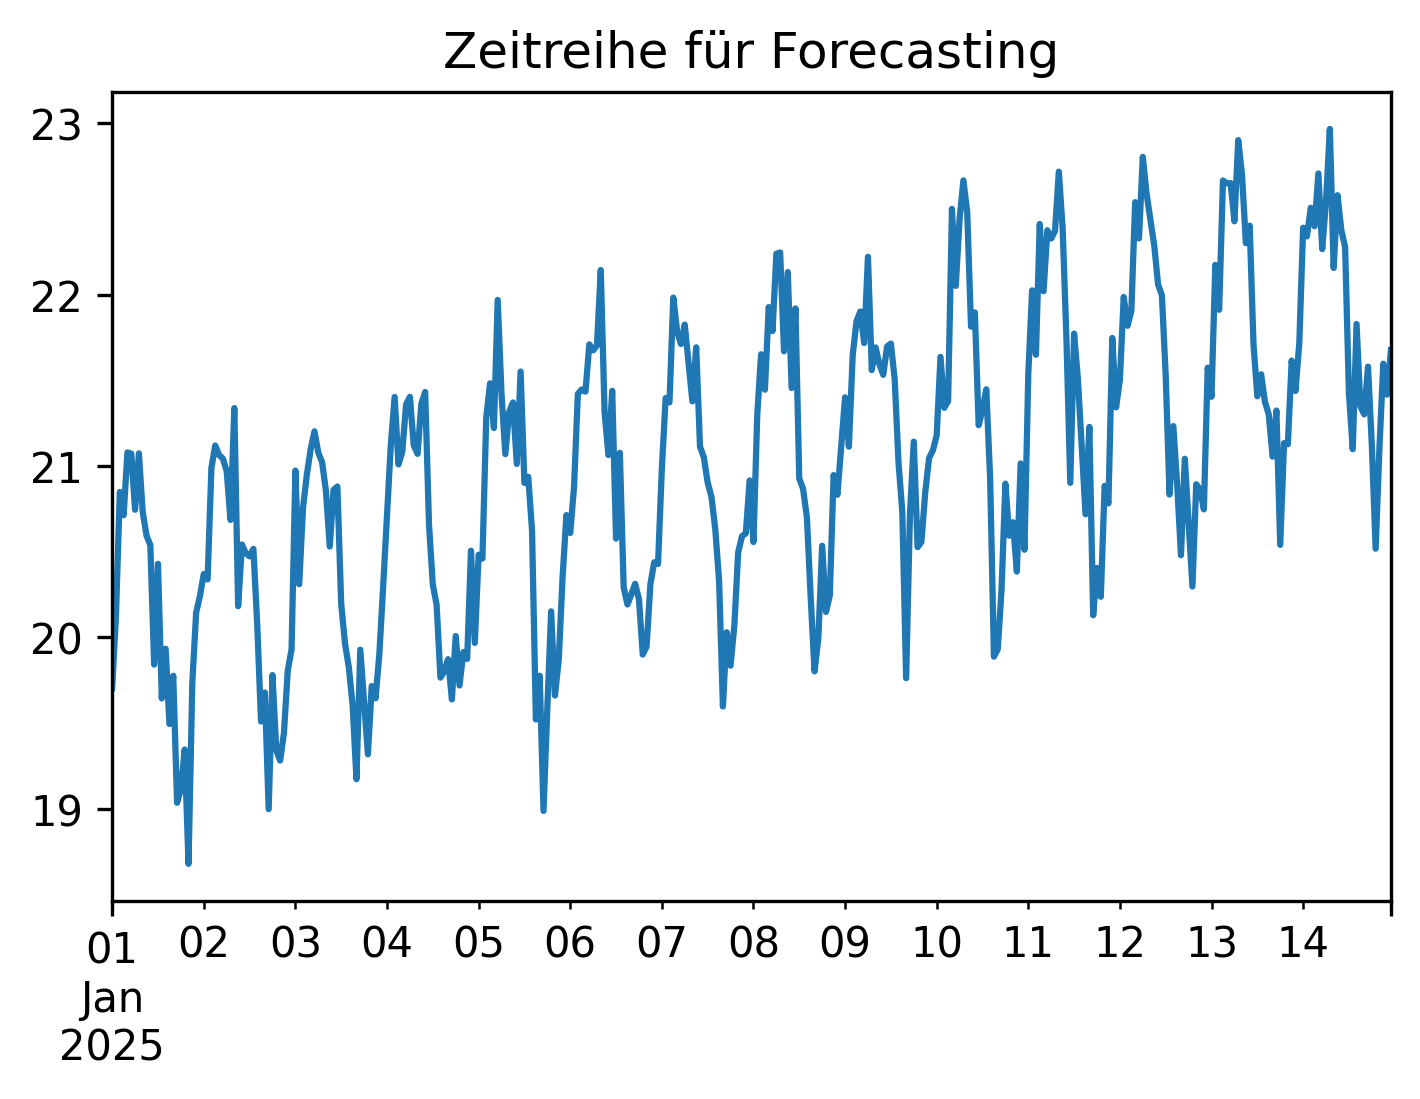
\includegraphics[keepaspectratio]{skript/08-forecasting-baselines_files/figure-pdf/cell-2-output-2.png}}

\begin{center}\rule{0.5\linewidth}{0.5pt}\end{center}

\section{8.2 Train-Test-Split}\label{train-test-split}

Wir verwenden 80\% der Daten für Training und 20\% für Test.

\begin{Shaded}
\begin{Highlighting}[]
\NormalTok{split }\OperatorTok{=} \BuiltInTok{int}\NormalTok{(}\BuiltInTok{len}\NormalTok{(s) }\OperatorTok{*} \FloatTok{0.8}\NormalTok{)}

\NormalTok{train }\OperatorTok{=}\NormalTok{ s.iloc[:split]}
\NormalTok{test }\OperatorTok{=}\NormalTok{ s.iloc[split:]}

\NormalTok{train.index.}\BuiltInTok{min}\NormalTok{(), train.index.}\BuiltInTok{max}\NormalTok{(), test.index.}\BuiltInTok{min}\NormalTok{(), test.index.}\BuiltInTok{max}\NormalTok{()}
\end{Highlighting}
\end{Shaded}

\begin{verbatim}
(Timestamp('2025-01-01 00:00:00'),
 Timestamp('2025-01-12 03:00:00'),
 Timestamp('2025-01-12 04:00:00'),
 Timestamp('2025-01-14 23:00:00'))
\end{verbatim}

\begin{center}\rule{0.5\linewidth}{0.5pt}\end{center}

\section{8.3 Naive Forecast}\label{naive-forecast}

Nächster Wert = letzter beobachteter Wert.

\section{Pandas}

\begin{Shaded}
\begin{Highlighting}[]
\NormalTok{naive }\OperatorTok{=}\NormalTok{ test.copy()}
\NormalTok{naive[:] }\OperatorTok{=}\NormalTok{ train.iloc[}\OperatorTok{{-}}\DecValTok{1}\NormalTok{]}
\end{Highlighting}
\end{Shaded}

\section{NumPy}

\begin{Shaded}
\begin{Highlighting}[]
\NormalTok{y }\OperatorTok{=}\NormalTok{ s.to\_numpy()}
\NormalTok{train\_np }\OperatorTok{=}\NormalTok{ y[:split]}
\NormalTok{test\_np }\OperatorTok{=}\NormalTok{ y[split:]}

\NormalTok{naive\_np }\OperatorTok{=}\NormalTok{ np.full\_like(test\_np, train\_np[}\OperatorTok{{-}}\DecValTok{1}\NormalTok{])}
\end{Highlighting}
\end{Shaded}

\begin{center}\rule{0.5\linewidth}{0.5pt}\end{center}

\section{8.4 Seasonal Naive (24
Stunden)}\label{seasonal-naive-24-stunden}

Nächster Wert = Wert von vor 24 Stunden.

\section{Pandas}

\begin{Shaded}
\begin{Highlighting}[]
\NormalTok{seasonal\_naive }\OperatorTok{=}\NormalTok{ s.shift(}\DecValTok{24}\NormalTok{).iloc[split:]}
\end{Highlighting}
\end{Shaded}

\section{NumPy}

\begin{Shaded}
\begin{Highlighting}[]
\NormalTok{seasonal\_naive\_np }\OperatorTok{=}\NormalTok{ y[split}\OperatorTok{{-}}\DecValTok{24}\NormalTok{:}\OperatorTok{{-}}\DecValTok{24}\NormalTok{]}
\end{Highlighting}
\end{Shaded}

\begin{center}\rule{0.5\linewidth}{0.5pt}\end{center}

\section{8.5 Moving Average Baseline}\label{moving-average-baseline}

Forecast = Mittelwert der letzten 24 Stunden.

\section{Pandas}

\begin{Shaded}
\begin{Highlighting}[]
\NormalTok{ma\_value }\OperatorTok{=}\NormalTok{ train.iloc[}\OperatorTok{{-}}\DecValTok{24}\NormalTok{:].mean()}
\NormalTok{ma\_forecast }\OperatorTok{=}\NormalTok{ test.copy()}
\NormalTok{ma\_forecast[:] }\OperatorTok{=}\NormalTok{ ma\_value}
\end{Highlighting}
\end{Shaded}

\section{NumPy}

\begin{Shaded}
\begin{Highlighting}[]
\NormalTok{ma\_value\_np }\OperatorTok{=}\NormalTok{ np.mean(train\_np[}\OperatorTok{{-}}\DecValTok{24}\NormalTok{:])}
\NormalTok{ma\_forecast\_np }\OperatorTok{=}\NormalTok{ np.full\_like(test\_np, ma\_value\_np)}
\end{Highlighting}
\end{Shaded}

\begin{center}\rule{0.5\linewidth}{0.5pt}\end{center}

\section{8.6 Vergleich visualisieren}\label{vergleich-visualisieren}

\begin{Shaded}
\begin{Highlighting}[]
\NormalTok{plt.figure()}
\NormalTok{train.plot(label}\OperatorTok{=}\StringTok{"Train"}\NormalTok{)}
\NormalTok{test.plot(label}\OperatorTok{=}\StringTok{"Test"}\NormalTok{)}
\NormalTok{naive.plot(label}\OperatorTok{=}\StringTok{"Naive"}\NormalTok{)}
\NormalTok{seasonal\_naive.plot(label}\OperatorTok{=}\StringTok{"Seasonal Naive"}\NormalTok{)}
\NormalTok{ma\_forecast.plot(label}\OperatorTok{=}\StringTok{"MA(24)"}\NormalTok{)}
\NormalTok{plt.legend()}
\NormalTok{plt.title(}\StringTok{"Forecast Baselines"}\NormalTok{)}
\NormalTok{plt.show()}
\end{Highlighting}
\end{Shaded}

\pandocbounded{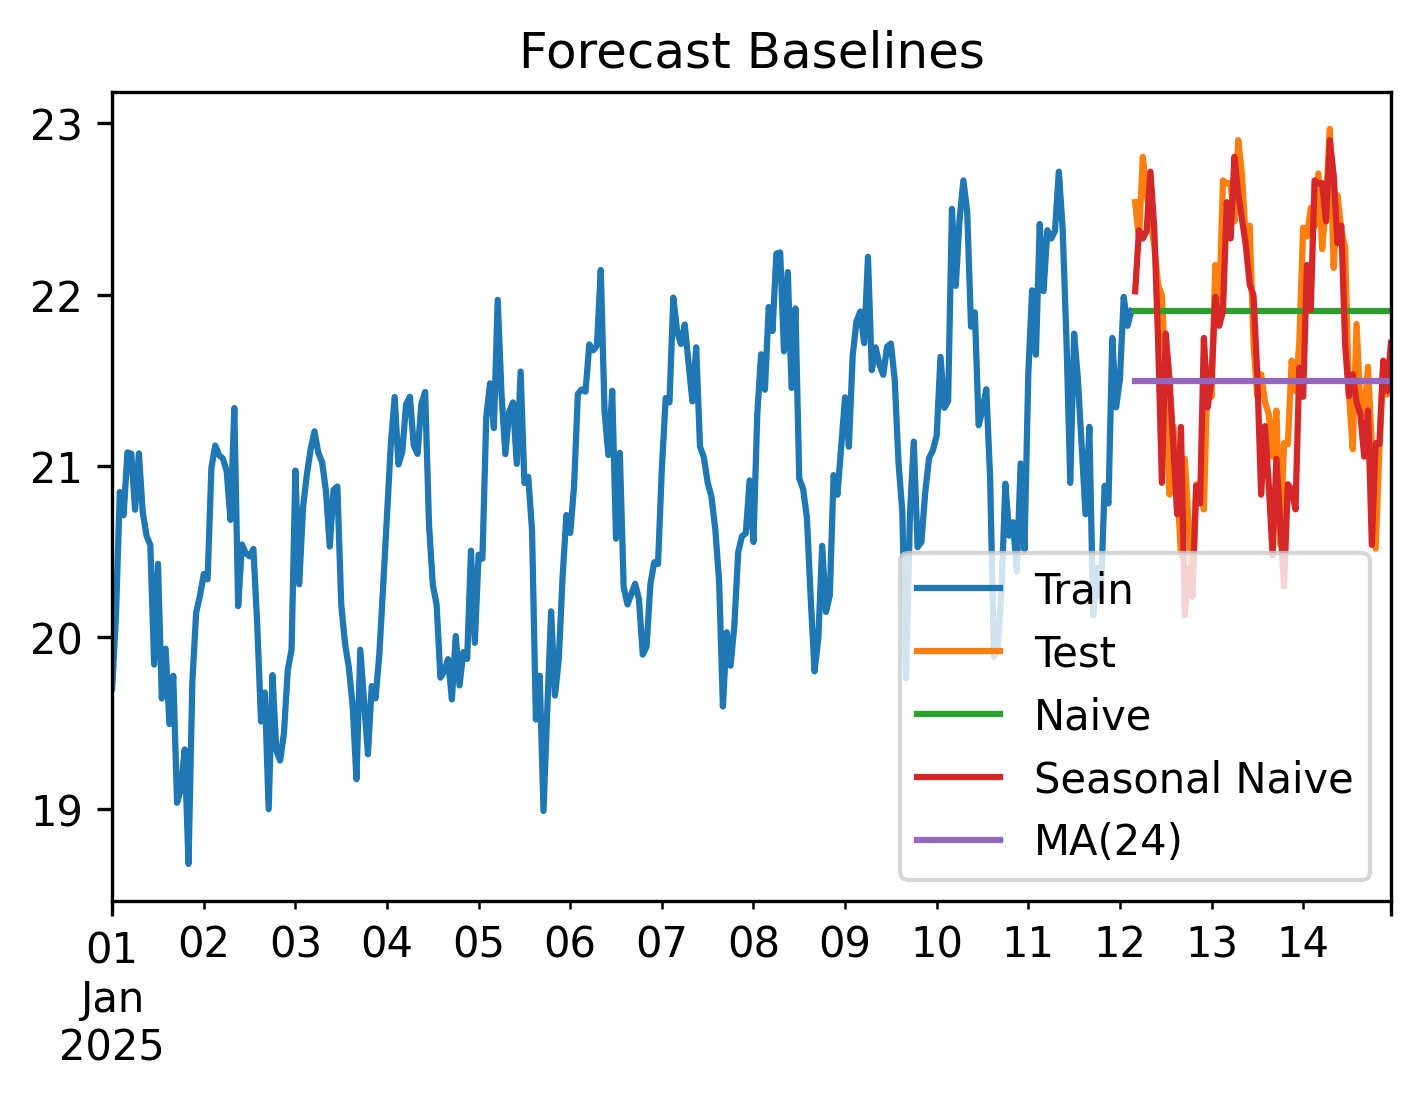
\includegraphics[keepaspectratio]{skript/08-forecasting-baselines_files/figure-pdf/cell-10-output-1.png}}

\begin{center}\rule{0.5\linewidth}{0.5pt}\end{center}

\section{8.7 Fehlermaße}\label{fehlermauxdfe}

Wir verwenden den Mean Absolute Error (MAE):

{[} MAE = \frac{1}{n} \sum \textbar y\_\{true\} - y\_\{pred\}\textbar{}
{]}

\section{Pandas}

\begin{Shaded}
\begin{Highlighting}[]
\KeywordTok{def}\NormalTok{ mae(y\_true, y\_pred):}
    \ControlFlowTok{return}\NormalTok{ np.mean(np.}\BuiltInTok{abs}\NormalTok{(y\_true }\OperatorTok{{-}}\NormalTok{ y\_pred))}

\BuiltInTok{print}\NormalTok{(}\StringTok{"MAE Naive:"}\NormalTok{, mae(test, naive))}
\BuiltInTok{print}\NormalTok{(}\StringTok{"MAE Seasonal Naive:"}\NormalTok{, mae(test, seasonal\_naive))}
\BuiltInTok{print}\NormalTok{(}\StringTok{"MAE MA(24):"}\NormalTok{, mae(test, ma\_forecast))}
\end{Highlighting}
\end{Shaded}

\begin{verbatim}
MAE Naive: 0.6298837368696829
MAE Seasonal Naive: 0.3320412574311427
MAE MA(24): 0.6228787570177815
\end{verbatim}

\section{NumPy}

\begin{Shaded}
\begin{Highlighting}[]
\KeywordTok{def}\NormalTok{ mae\_np(y\_true, y\_pred):}
    \ControlFlowTok{return}\NormalTok{ np.mean(np.}\BuiltInTok{abs}\NormalTok{(y\_true }\OperatorTok{{-}}\NormalTok{ y\_pred))}

\BuiltInTok{print}\NormalTok{(}\StringTok{"MAE Naive:"}\NormalTok{, mae\_np(test\_np, naive\_np))}
\BuiltInTok{print}\NormalTok{(}\StringTok{"MAE Seasonal:"}\NormalTok{, mae\_np(test\_np, seasonal\_naive\_np))}
\BuiltInTok{print}\NormalTok{(}\StringTok{"MAE MA(24):"}\NormalTok{, mae\_np(test\_np, ma\_forecast\_np))}
\end{Highlighting}
\end{Shaded}

\begin{verbatim}
MAE Naive: 0.6298837368696829
MAE Seasonal: 0.3320412574311427
MAE MA(24): 0.6228787570177815
\end{verbatim}

\begin{center}\rule{0.5\linewidth}{0.5pt}\end{center}

\section{8.8 Interpretation}\label{interpretation}

Typische Beobachtungen:

\begin{itemize}
\tightlist
\item
  Bei starker Saison gewinnt häufig Seasonal Naive.
\item
  Bei schwachem Muster ist Naive oft überraschend stark.
\item
  Moving Average glättet, reagiert aber träge auf Trendänderungen.
\end{itemize}

\begin{center}\rule{0.5\linewidth}{0.5pt}\end{center}

\begin{tcolorbox}[enhanced jigsaw, titlerule=0mm, title=\textcolor{quarto-callout-tip-color}{\faLightbulb}\hspace{0.5em}{Methodischer Hinweis}, bottomrule=.15mm, opacityback=0, colbacktitle=quarto-callout-tip-color!10!white, coltitle=black, opacitybacktitle=0.6, colframe=quarto-callout-tip-color-frame, toprule=.15mm, leftrule=.75mm, arc=.35mm, rightrule=.15mm, breakable, bottomtitle=1mm, colback=white, toptitle=1mm, left=2mm]

Baseline-Vergleich ist keine Formalität, sondern eine
Qualitätskontrolle.

\end{tcolorbox}

\begin{center}\rule{0.5\linewidth}{0.5pt}\end{center}

\section{8.9 Mini-Aufgaben}\label{mini-aufgaben-4}

\begin{enumerate}
\def\labelenumi{\arabic{enumi}.}
\tightlist
\item
  Erhöhen Sie die Stärke der Saison.

  \begin{itemize}
  \tightlist
  \item
    Welche Baseline gewinnt?
  \end{itemize}
\item
  Entfernen Sie die Saison vollständig.

  \begin{itemize}
  \tightlist
  \item
    Welche Baseline wird besser?
  \end{itemize}
\item
  Fügen Sie einen starken Trend hinzu.

  \begin{itemize}
  \tightlist
  \item
    Wie reagieren die Modelle?
  \end{itemize}
\end{enumerate}

\bookmarksetup{startatroot}

\chapter{9 Lernzielkontrolle}\label{lernzielkontrolle}

\bookmarksetup{startatroot}

\chapter{9 Lernzielkontrolle}\label{lernzielkontrolle-1}

Nutzen Sie diese Checkliste zur Selbstüberprüfung.

\begin{center}\rule{0.5\linewidth}{0.5pt}\end{center}

\section{9.1 Fachliche Kompetenzen}\label{fachliche-kompetenzen}

Ich kann \ldots{}

\begin{itemize}
\tightlist
\item[$\square$]
  eine Zeitreihe methodisch einordnen (Messprozess, Abtastrate).
\item[$\square$]
  eine Zeitreihe validieren (Sortierung, Duplikate, Missing Values).
\item[$\square$]
  Resampling begründet einsetzen (Aggregation vs.~Interpolation).
\item[$\square$]
  Rolling Mean und EWMA unterscheiden und passend wählen.
\item[$\square$]
  Trend und Saison konzeptionell trennen.
\item[$\square$]
  Lag-Features erzeugen und interpretieren.
\item[$\square$]
  Autokorrelation interpretieren.
\item[$\square$]
  Anomalien global und lokal definieren.
\item[$\square$]
  Baseline-Forecasts implementieren.
\item[$\square$]
  Forecast-Modelle mit MAE bewerten.
\end{itemize}

\begin{center}\rule{0.5\linewidth}{0.5pt}\end{center}

\section{9.2 Verständnisfragen}\label{verstuxe4ndnisfragen}

\begin{enumerate}
\def\labelenumi{\arabic{enumi}.}
\tightlist
\item
  Warum ist die Abtastrate für die Interpretation einer Saison
  entscheidend?
\item
  Wann ist Interpolation problematisch?
\item
  Warum kann ein Trend die Autokorrelation künstlich erhöhen?
\item
  Warum sind Baselines methodisch wichtig?
\item
  Wodurch unterscheidet sich ein Strukturbruch von einem Ausreißer?
\end{enumerate}

\begin{center}\rule{0.5\linewidth}{0.5pt}\end{center}

\begin{tcolorbox}[enhanced jigsaw, titlerule=0mm, title=\textcolor{quarto-callout-tip-color}{\faLightbulb}\hspace{0.5em}{Hinweis}, bottomrule=.15mm, opacityback=0, colbacktitle=quarto-callout-tip-color!10!white, coltitle=black, opacitybacktitle=0.6, colframe=quarto-callout-tip-color-frame, toprule=.15mm, leftrule=.75mm, arc=.35mm, rightrule=.15mm, breakable, bottomtitle=1mm, colback=white, toptitle=1mm, left=2mm]

Wenn mehrere Punkte unsicher sind, wiederholen Sie gezielt die
entsprechenden Kapitel und bearbeiten Sie die Übungsaufgaben.

\end{tcolorbox}

\bookmarksetup{startatroot}

\chapter{10 Übung:
Zeitreihen-Workflow}\label{uxfcbung-zeitreihen-workflow}

\bookmarksetup{startatroot}

\chapter{10 Übung:
Zeitreihen-Workflow}\label{uxfcbung-zeitreihen-workflow-1}

Diese Übung kombiniert mehrere Methoden aus dem Baustein.

\begin{center}\rule{0.5\linewidth}{0.5pt}\end{center}

\section{Aufgabe 1: Eigene Zeitreihe
erzeugen}\label{aufgabe-1-eigene-zeitreihe-erzeugen}

Erzeugen Sie eine Zeitreihe mit:

\begin{itemize}
\tightlist
\item
  10 Tagen, stündlicher Abtastrate
\item
  Trend
\item
  Tages-Saison
\item
  Rauschen
\item
  mindestens 3 Anomalien
\end{itemize}

Visualisieren Sie die Zeitreihe.

\begin{center}\rule{0.5\linewidth}{0.5pt}\end{center}

\section{Aufgabe 2: Validierung}\label{aufgabe-2-validierung}

Bauen Sie absichtlich Fehler ein:

\begin{itemize}
\tightlist
\item
  Duplikate
\item
  Missing Values
\item
  Unsortierte Zeitpunkte
\end{itemize}

Implementieren Sie eine saubere Validierung.

\begin{center}\rule{0.5\linewidth}{0.5pt}\end{center}

\section{Aufgabe 3: Resampling}\label{aufgabe-3-resampling}

\begin{itemize}
\tightlist
\item
  Aggregieren Sie auf Tagesmittel.
\item
  Vergleichen Sie Original und Aggregation.
\item
  Interpretieren Sie Informationsverlust.
\end{itemize}

\begin{center}\rule{0.5\linewidth}{0.5pt}\end{center}

\section{Aufgabe 4: Glättung}\label{aufgabe-4-gluxe4ttung}

\begin{itemize}
\tightlist
\item
  Testen Sie Rolling-Fenster von 6H, 24H, 72H.
\item
  Welche Struktur wird jeweils sichtbar?
\end{itemize}

\begin{center}\rule{0.5\linewidth}{0.5pt}\end{center}

\section{Aufgabe 5: Anomalien}\label{aufgabe-5-anomalien}

\begin{itemize}
\tightlist
\item
  Implementieren Sie eine EWMA-Baseline.
\item
  Detektieren Sie Anomalien.
\item
  Variieren Sie den Schwellenwert.
\end{itemize}

\begin{center}\rule{0.5\linewidth}{0.5pt}\end{center}

\section{Aufgabe 6:
Forecast-Baselines}\label{aufgabe-6-forecast-baselines}

\begin{itemize}
\tightlist
\item
  Train-Test-Split (80/20)
\item
  Naive
\item
  Seasonal Naive (24H)
\item
  MA(24)
\end{itemize}

Vergleichen Sie die MAE-Werte und interpretieren Sie das Ergebnis.

\begin{center}\rule{0.5\linewidth}{0.5pt}\end{center}

\begin{tcolorbox}[enhanced jigsaw, titlerule=0mm, title=\textcolor{quarto-callout-note-color}{\faInfo}\hspace{0.5em}{Abgabeformat (optional)}, bottomrule=.15mm, opacityback=0, colbacktitle=quarto-callout-note-color!10!white, coltitle=black, opacitybacktitle=0.6, colframe=quarto-callout-note-color-frame, toprule=.15mm, leftrule=.75mm, arc=.35mm, rightrule=.15mm, breakable, bottomtitle=1mm, colback=white, toptitle=1mm, left=2mm]

Plots + kurze Interpretation (Stichpunkte).

\end{tcolorbox}

\bookmarksetup{startatroot}

\chapter{11 Klausurfragen}\label{klausurfragen}

\bookmarksetup{startatroot}

\chapter{11 Klausurfragen}\label{klausurfragen-1}

\section{Verständnisfragen}\label{verstuxe4ndnisfragen-1}

\begin{enumerate}
\def\labelenumi{\arabic{enumi}.}
\tightlist
\item
  Definieren Sie eine Zeitreihe.
\item
  Was ist der Unterschied zwischen Aggregation und Interpolation?
\item
  Erklären Sie Rolling Mean und EWMA konzeptionell.
\item
  Was ist ein Lag-Feature?
\item
  Was misst die Autokorrelation?
\item
  Warum kann Trend die Autokorrelation beeinflussen?
\item
  Erklären Sie den Unterschied zwischen globaler und lokaler
  Anomalie-Detektion.
\item
  Was ist eine Forecast-Baseline?
\item
  Warum sind Baselines methodisch notwendig?
\item
  Was misst der MAE?
\end{enumerate}

\begin{center}\rule{0.5\linewidth}{0.5pt}\end{center}

\section{Transferfragen}\label{transferfragen}

\begin{enumerate}
\def\labelenumi{\arabic{enumi}.}
\tightlist
\item
  Sie erhalten Maschinendaten mit starker Wochenperiodik.

  \begin{itemize}
  \tightlist
  \item
    Welche Schritte würden Sie durchführen?
  \end{itemize}
\item
  Eine Zeitreihe zeigt plötzlich dauerhaft höhere Werte.

  \begin{itemize}
  \tightlist
  \item
    Ausreißer oder Strukturbruch? Begründen Sie.
  \end{itemize}
\item
  Zwei Zeitreihen sollen verglichen werden, eine minütlich, eine
  stündlich gemessen.

  \begin{itemize}
  \tightlist
  \item
    Welche Schritte sind notwendig?
  \end{itemize}
\end{enumerate}

\begin{center}\rule{0.5\linewidth}{0.5pt}\end{center}

\begin{tcolorbox}[enhanced jigsaw, titlerule=0mm, title=\textcolor{quarto-callout-warning-color}{\faExclamationTriangle}\hspace{0.5em}{Hinweis zur Prüfungsvorbereitung}, bottomrule=.15mm, opacityback=0, colbacktitle=quarto-callout-warning-color!10!white, coltitle=black, opacitybacktitle=0.6, colframe=quarto-callout-warning-color-frame, toprule=.15mm, leftrule=.75mm, arc=.35mm, rightrule=.15mm, breakable, bottomtitle=1mm, colback=white, toptitle=1mm, left=2mm]

Begründen Sie Ihre Antworten stets methodisch. Reine Definitionen
reichen meist nicht aus.

\end{tcolorbox}




\end{document}
